\documentclass[%
candidate, % тип документа
subf, % подключить и настроить пакет subfig для вложенной нумерации рисунков
%href, % подключить и настроить пакет hyperref
%colorlinks=true % цветные гиперссылки
times % шрифт Times как основной
%,fixint=false % отключить прямые знаки интегралов
]{disser}

\usepackage[
a4paper, mag=1000,
left=2.5cm, right=1cm, top=2cm, bottom=2cm, headsep=0.7cm, footskip=1cm
]{geometry}
\usepackage[T2A]{fontenc}
%\usepackage{cite}
\usepackage[utf8]{inputenc}
\usepackage[english,russian]{babel}
\usepackage{pdfpages}
\ifpdf\usepackage{epstopdf}\fi

\usepackage{dcolumn}
\usepackage{bm}
\usepackage{hyperref}
\usepackage{color}
\usepackage{epstopdf}
\usepackage{amsmath}
\usepackage{amssymb}
\usepackage{cite}
\usepackage{multirow}
\usepackage{afterpage}
\usepackage[font={normal}]{caption}

\usepackage{setspace}

%\usepackage{fancyhdr}
%\pagestyle{fancy}

\captionsetup{format=hang,labelsep=period}

% Использовать полужирное начертание для векторов
\let\vec=\mathbf

% Включать подсекции в оглавление
\setcounter{tocdepth}{2}

\graphicspath{{Ris/}}

\bibliographystyle{unsrt}

\begin{document}
%\includepdf[pages={1-1}]{NIRS.pdf}
% Содержание


\begin{titlepage}

\begin{center}
{
\footnotesize\setstretch{1.0}
Федеральное государственное бюджетное образовательное учреждение высшего образования\\
<<Московский государственный технический университет имени Н.Э. Баумана\\ (национальный исследовательский университет)>>\\(МГТУ им. Н.Э. Баумана)\\
}
\end{center}
\begin{figure}[h!]
% \begin{minipage}[b]{0.2\textwidth}\centering
%\begin{flushright}
% \includegraphics[width=0.9\linewidth]{r2.png}
%\end{flushright}
% \end{minipage}
\begin{minipage}[b]{0.9\textwidth}\setstretch{1.5}\centering
Факультет <<Фундаментальные науки>>\\
Кафедра <<Физика>> ФН4
\\\vspace{1.5cm}
\end{minipage}
\end{figure}
\begin{flushright}
На правах рукописи\\
УДК 538.9
\end{flushright}

\vspace{10mm}

\begin{center}
\textbf{НАУЧНО-КВАЛИФИКАЦИОННАЯ РАБОТА}\\\vspace{5mm}
\textbf{<<Роль дальнодействия притяжения в фазовых диаграммах и диффузии в двумерных системах с регулируемыми взаимодействиями>>}
\end{center}


\vspace{5mm}

\begin{flushleft}
Направление подготовки: 03.06.01 Физика и астрономия\\
Направленность (профиль): 01.04.07 Физика конденсированного состояния
\end{flushleft}

\vspace{5mm}

\begin{table}[h]
\begin{tabular}{lll}
Студент\hspace{4cm} & \underline{\hspace{4cm}} & \hspace{2cm}Дмитрюк Н.А.\\\\
Научный руководитель\\д.ф.-м.н. & \underline{\hspace{4cm}} & \hspace{2cm}Юрченко С.О.
\end{tabular}
\end{table}

\vspace{40mm}

\begin{center}
Москва -- 2020
\end{center}
\end{titlepage}

%\nocite{10.1103/PhysRevLett.121.075003, 10.1039/c8sm01836g, 10.1063/1.4979325, 10.1039/C7SM02429K, 10.1063/1.5082785, 10.1063/1.4926945, 10.1088/0953-8984/28/23/235401, 10.1063/1.5022969, 10.1063/1.4921223, 10.1103/PhysRevE.97.022616, 10.1021/acs.langmuir.6b01644, 10.1103/PhysRevE.96.043201, 10.1063/1.5050708, 10.3367/ufnr.2019.01.038520, 10.1063/1.5088141, 10.1364/FIO.2016.FTh4C.2, 10.1088/1742-6596/1135/1/012093}
\onehalfspacing
\setcounter{page}{2}
\tableofcontents
%\addtocontents{toc}{~\hfill\textbf{Стр.}\par}
%\addtocontents{toc}{~\hfill\textbf{Стр.}\par}
%\addtocontents{toc}{\protect\afterpage{~\hfill\textbf{Стр.}\par\medskip}}
%\addtocontents{toc}{\protect\afterpage{\protect\afterpage{~\hfill\textbf{Стр.}\par\medskip}}}


%\chapter*{Введение}
%\addcontentsline{toc}{chapter}{Введение}

\newpage
\begin{center}
\textbf{ВВЕДЕНИЕ}
\end{center}
%\refstepcounter{chapter}
\addcontentsline{toc}{chapter}{ВВЕДЕНИЕ}



\textbf{Актуальность.}

Для физики конденсированного состояния большой интерес представляют такие явления, как кристаллизация, плавление, критические явление, а так же их зависимость от свойств системы. Понимание влияния этих свойств на систему играет важную роль в материаловедении.


На данный момент эти проблемы решаются с использованием математических моделей систем.



\textbf{Цель работы} --
установить связь между дальнодействием притяжения в двумерной системе частиц, взаимодействующих посредством обобщенного потенциала Леннарда-Джонса, c фазовой диаграммой, и параметрами переноса.

\textbf{Задачи работы:}
\begin{enumerate}
\item Разработка программного комплекса для расчета явлений переноса в $2D$ системах.
\item Разработка методов определения термодинамических свойств системы по распределениям плотностей. 
\item Усовершенствование метода распознавание фаз и построения фазовых диаграмм.
\item Применение разработанных методов на различных потенциалах взаимодействия.
\item Применение наработок для изучения влияния потенциала взаимодействия на различные термодинамические параметры.
\end{enumerate}

\textbf{Научная новизна работы:}
\begin{enumerate}
\item Впервые показано, что термодинамические свойства системы могут быть рассчитаны по распределению статических параметров.

\end{enumerate}

\textbf{Положения, выносимые на защиту:}
\begin{enumerate}
\item Показано, что ...

\item Показано, что ...

\item Показано, что ...

\end{enumerate}

\textbf{Методология и методы исследования.} 
Сформулированные задачи были решены с помощью моделирования систем методами молекулярной динамики, с использованием свободного программного пакета LAMMPS. Пост-обработка результатов выполнена с помощью разработанного программного комплекса на языке MATLAB и Python.


\textbf{Достоверность.} 

\textbf{Личный вклад автора.}

\textbf{Теоретической значимостью.} 

\textbf{Практическая значимость.} 

\textbf{Результат работы.} 

\textbf{Апробация работы.} 

\textbf{Публикации.} 
Основные результаты работы находятся на рецензировании.

\textbf{Структура и объем работы.} 
Научно квалификационная работа состоит из введения, 3 глав и заключения, содержит N страниц, N рисунков.
Список литературы включает N источников.

Во \textbf{введении} кратко обосновывается актуальность работы, формулируется цель, перечисляются положения, выносимых на защиту, указывается научная новизна, достоверность, фундаментальная и практическая значимость результатов работы, личный вклад автора, апробация работы и содержание по главам.


\textbf{Глава 1} является обзорной.
В разделе \ref{C1_1} кратко рассматриваются межмолекулярные взаимодействия.
В разделе \ref{C1_2} рассматриваются взаимодействия коллойдов в присутствии внешних полей.

В разделе \ref{C1_3} рассматриваются параметры переноса в веществе. 


\textbf{Глава 2} посвящена изучению роли дальнодействия притяжения в фазовых диаграммах.


В разделе \ref{C2_1} излагается метод разбиения системы на ячейки вороного.

В разделе \ref{C2_2} демонстрируется применение предложенного подхода на различных потенциалах взаимодействия.

В разделе \ref{C2_3} демонстрируется методы анализа гистограмм распределения плотностей различных потенциалах взаимодействия.

В разделе \ref{C2_4} \textbf{обобщаются основные результаты главы}.

\textbf{Глава 3} посвящена рассмотрению явлений переноса при разных потенциалах взаимодействия.

В разделе \ref{C3_1} рассматриваются методы измерения параметров переноса вещества на различных потенциалах взаимодействия.

В разделе \ref{C3_2} рассматриваются связь термодинамических параметров, и параметров переноса вещества.

В разделе \ref{C3_3} обобщаются основные результаты главы.

В \textbf{общих выводах и заключении} обобщаются основные результаты работы.
%\newpage
\newpage
%\chapter*{Введение}
%\addcontentsline{toc}{chapter}{Введение}

\newpage
\begin{center}
\textbf{ГЛАВА 1}\\
\textbf{НАЗВАНИЕ ПЕРВОЙ ГЛАВЫ}
\end{center}
\refstepcounter{chapter}


% \section*{}
\addcontentsline{toc}{chapter}{ГЛАВА 1. Название первой главы}


\section{Межмолекулярные взаимодействия}\label{C1_1}

К межмолекулярным взаимодействиям относятся взаимодействия между молекулами и/или атомами, не приводящие к образованию ковалентных химических связей.

Межмолекулярные взаимодействия имеют электростатическую природу. На больших расстояниях преобладают силы притяжения, которые могут иметь ориентационную, поляризационную и дисперсионную природу.

В случае коллоидных частиц, как правило, из-за разного материала частиц и сольвента возникает притяжение Ван-дер-Ваальса [31, 53!!]

\begin{equation}
\varphi_{\mathrm{vdW}}(r)=-\frac{A_{\mathrm{H}}}{12}\left(\frac{\sigma^{2}}{r^{2}-\sigma^{2}}+\frac{\sigma^{2}}{r^{2}}+2 \ln \frac{r^{2}-\sigma^{2}}{r^{2}}\right)
\end{equation}
где постоянная Хамакера $A_{\mathrm{H}} \propto\left(\frac{\varepsilon_{\mathrm{r}}-1}{\varepsilon_{\mathrm{r}}+1}\right)^{2}$ зависит от относительной диэлектрической проницаемости $\varepsilon_{\mathrm{r}}=\varepsilon_{\mathrm{P}} / \varepsilon_{\mathrm{S}}$. 

Для предотвращения коагуляции в коллоидной системе присутствуют силы отталкивания, которые обусловлены зарядовой или стерической стабилизацией.

Зарядовая стабилизация возникает благодаря взаимному отталкиванию заряженных частиц, в результате накопленного на их поверхности отрицательного заряда, который возникает при диссоциации поверхности и адсорбции ионов. 
В рамках линеаризованной теории Пуассона-Больцмана, взаимодействие Дерягина-Ландау-Фервея-Овербека имеет вид [54!!]
\begin{equation}
\varphi_{Y}(r)=\left\{\begin{array}{ll}
\infty & r<\sigma, \\
\epsilon_{\mathrm{Y}} \frac{e^{-\kappa(r-\sigma)}}{r / \sigma} & r \geq \sigma,
\end{array}\right.
\end{equation}

где $\kappa=\sqrt{4 \pi \lambda_{\mathrm{B}} n_{\mathrm{ion}}} \equiv \lambda_{\mathrm{D}}^{-1}$ - обратная дебаевская длина экранирования, выраженная через плотность малых ионов $n_{ion}$ и длину Бьеррума $\lambda_{\mathrm{B}}=e^{2} / \varepsilon_{\mathrm{w}} k_{\mathrm{B}} T$. Контактный потенциал записывается как 

\begin{equation}
\epsilon_{\mathrm{Y}}=\frac{Z^{2}}{(1+\kappa \sigma / 2)^{2}} \frac{\lambda_{\mathrm{B}}}{\sigma} k_{\mathrm{B}} T,
\end{equation}
где $Z \equiv Q / e$ зарядовое число коллоида.

Результирующее взаимодействие представляет собой сумму притягивающих и отталкивающих сил:
\begin{equation}
\varphi(r)=\varphi_{Y}(r)+\varphi_{\mathrm{vdW}}(r).
\end{equation}
Вклады данных слагаемых соизмеримы на малом расстоянии между не сильно заряженными частицами.

С ростом заряда частиц, теория Пуассона-Больцмана становится неприменимой вблизи поверхности частицы, однако на дальних расстояния по прежнему имеет форму Юкавы, и при ренормированном зарядом может хорошо описывать потенциал вдали от поверхности [55]. Эффективный насыщенный заряд выражается следующим уравнением [56]
\begin{equation}
Z_{\mathrm{eff}}^{\mathrm{sat}}=(2+\kappa \sigma) \sigma / \lambda_{\mathrm{B}}
\end{equation}
Используя линеаризованную теорию Пуассона - Больцмана с установленным эффективным зарядом, можно объяснить большинство экспериментальных наблюдений [57-59]. Это делает теорию Дерягина-Ландау-Фервея-Овербека (ДЛФО) одним из наиболее успешных подходов при описании межчастичных взаимодействий [49, 60, 61]. 

Помимо зарядовой стабилизации существует так называемая стерическая стабилизация. Она заключается в добавлении в сольвент полимерных молекул, которые оседают на частицах. При сближении частиц, эти полимерные цепи взаимодействуют друг с другом, не давая частицам сблизиться сильнее. 

Часть потенциала взаимодействия, которая соответствует стерической стабилизации, выглядит следующим образом [31]
\begin{equation}
\begin{array}{l}
\varphi_{\text {steric }}(r)=\frac{\pi \sigma}{2} \int_{r-\sigma}^{\infty} d h F(h) \\
\\
F(r)=\frac{\alpha k_{\mathrm{B}} T}{s^{3}}\left[\left(\frac{2 L}{r}\right)^{9 / 4}-\left(\frac{r}{2 L}\right)^{3 / 4}\right], \quad r<2 L
\end{array}
\label{eqStericStabl}
\end{equation}
где $L$ - толщина полимерного слоя, $\alpha$ - численный множитель, определяемый для конкретных полимеров
особенностями взаимодействия между молекулярными цепочками, $s$ - среднее расстояние между привитыми полимерами на поверхности.

В случае наличия этих взаимодействий, суммарный потенциал частиц выражается следующей формулой

\begin{equation}
\varphi(r)=\varphi_{Y}(r)+\varphi_{\mathrm{vdW}}(r)+\varphi_{\mathrm{steric}}(r).
\end{equation}

Для изучения влияния микроскопических свойств на макроскопические свойства, используется так называемый метод молекулярной динамики, который заключается в численном моделировании системы, состоящей из достаточно большого количества частиц, по статистике которых можно судить о макроскопических свойствах. Одним из наиболее популярных модельных потенциалов взаимодействия частиц в таких системах, является потенциал Леннарда - Джонса 
\begin{equation}
U\left(R_{i j}\right)=\varepsilon\left[\left(\frac{R_{0}}{R_{i j}}\right)^{12}-2\left(\frac{R_{0}}{R_{i j}}\right)^{6}\right]=4 \varepsilon\left[\left(\frac{\sigma}{R_{i j}}\right)^{12}-\left(\frac{\sigma}{R_{i j}}\right)^{6}\right], 
\label{eqFullLJ}
\end{equation}
где $\varepsilon$ и $R_0$ - глубина потенциальной ямы и равновесное расстояние между частицами; $R_0 = 2^{1/6}\sigma$.

В то время как зависимость $R^{-6}$ получена теоретически и обусловлена силами Ван-дер-Ваальса, зависимость $R^{-12}$ выбрана из соображений удобства.

Различные физические величины в данных моделированниях удобно выражать через константы моделирования $\sigma, \varepsilon, m$.

Метод молекулярной динамики (МД) позволяет в данной работе выяснить влияние дальнодействия притяжения на термодинамические свойства системы и параметры переноса.

\section{Регулируемые межчастичные взаимодействия}\label{C1_2}



\section{Цели и задачи работы}

\textbf{Цель бакалаврской работы}:

установить связь между дальнодействием притяжения в двумерной системе частиц, взаимодействующих посредством обобщенного потенциала Леннарда-Джонса, и фазовой диаграммой, а также параметров переноса.

\newpage
%\chapter*{Введение}
%\addcontentsline{toc}{chapter}{Введение}

\newpage
\begin{center}
\textbf{ГЛАВА 2}\\
\textbf{КОЛЛЕКТИВНЫЕ СПЕКТРЫ В КОНДЕНСИРОВАННЫХ СИСТЕМАХ}
\end{center}
\refstepcounter{chapter}


% \section*{}
\addcontentsline{toc}{chapter}{ГЛАВА 1. Коллективные спектры в конденсированных системах}
\section{Расчет спектров в МД}

%Значительное число ключевых свойств конденсированного вещества определяется спектрами элементарных возбуждений и, в частности, коллективных колебаний. Однако поведение и описание коллективных мод в неупорядоченных средах (например, жидкостях и стеклах) остается сложной областью современной науки о конденсированных средах. В последнее время теоретически предсказывалось и наблюдалось в молекулярно-динамическом моделировании антикроссинга между продольными и поперечными модами, но это фундаментальное явление никогда не наблюдалось экспериментально. 

Коллективные возбуждения являются одной из ключевых концепций современной
физики конденсированного состояния ~\cite{dove_1993, HansenMacDonald, landau.statphys}. Это обусловлено тем,
что знание коллективных возбуждений в конденсированной системе позволяет
понять многие свойства системы, такие как: термодинамические, упругие,
структурные и т.д. Коллективные возбуждения в случае кристаллических систем
являются наиболее изученными. Главным образом благодаря наличию
трансляционной симметрии и малости отклонений частиц кристаллической решетки
от положений равновесия. Трансляционная симметрия позволяет рассматривать
коллективные возбуждения в кристалле как плоские волны, а малость
отклонений позволяет рассматривать как гармонические невзаимодействующие
колебания. В физике твердого данные колебания принято отождествлять
с квазичастицами - фононами. При высоких температурах отклонения
частиц становятся большими и фононы уже нельзя рассматривать как невзаимодействующие.


В случае жидкостей так же можно говорить о коллективных возбуждениях,
однако они имеют более сложную структуру и хуже изучены. Однако
существует теоретический подход к оценке дисперсионных зависимостей в жидкостях,
известный, как QCA (quasi-crystalline approximation) ~\cite{Khrapak:2018aa}. Во многих
случаях описание на основе QCA справедливо и согласуется с дисперсионными
кривыми, полученными экспериментально, для различных простых жидкостей,
по крайней мере.


В контексте физики плазмы первоначально был предложен аналог QCA -- подход QLCA (quasi-localized charge approximation) ~\cite{doi:10.1063/1.873814}, который использовался для расчета дисперсии  коллективных мод в  сильно коррелированной жидкой фазе.
%случае различных кулоновских систем, бинарных ионых смесей, электронных бислоев, однокомпонентной системы Юкавы в

Метод был создан для сильно связанных систем, где традиционная аппроксимация рандомной фазы RPA (random-phase approximation) или иерархия ББГКИ не была бы оправдана. Теория QLCA позволила предсказать дисперсию плазменных и сдвиговых мод не только в упомянутых выше системах, но и в намагниченной однокомпонентной плазме и в электронных сверхрешетках.

Подход QCA связывает динамические и структурные характеристики системы,
то есть позволяет рассчитать дисперсионные соотношения для коллективных
возбуждений в жидкости, на основе потенциальной энергии парного взаимодействия
и парной-корреляционной функции $g(r)$.
Однако обратная процедура плохо изучена, и теория восстановления парных
корреляций с использованием потенциала взаимодействия и динамических свойств
хорошо развита только для кристаллов \cite{10.1039/C7SM02429K, Khrapak:Practicalth, Yurchenko2016IM}.

Для анализа различных подходов к построению спектров элементарных возбуждений было проведено моделирование на основе методов молекулярной динамики (МД) с использованием NVT ансамбля.
Рассматривался метод построения на основе простых жидкостей с потенциалами Леннарда-Джонса и Юкавы:

\begin{equation}
\varphi_{LJ} = 4 \varepsilon \Big[\Big(\frac{\lambda}{r} \Big)^{12} - \Big(\frac{\lambda}{r} \Big)^6\Big],
\end{equation}

\begin{equation}
\varphi_{Y} = \varepsilon \frac{\lambda}{r} \Big(-\frac{r}{\lambda} \Big),
\label{Yukawa}
\end{equation}


где $\varepsilon$ и $\lambda$ – магнитуда и характерная длина взаимодействия соответственно.

В случае систем с потенциалом Леннарда-Джонса система состояла из $N = 10^4$ частиц с радиусом отсечки $r_c = 7.5 n^{-1/D}$, где $n = N/V$ - плотность, а $D$ - размерность системы. Моделирования проводились с временным шагом $\Delta t = 5 \times 10^{-3} \sqrt{T_0 m \sigma^2/(T\epsilon)}$.



Для рассмотренной системы на основе данных, полученных в результате моделирования, были рассчитаны плотности потока скоростей на основе фурье-преобразования \cite{Khrapak:2018aa}:\\
\begin{equation}
C_{L, T}(q, \omega) = \int dt e^{i\omega t} Re \langle \mathbf{j}_{L,T} (\mathbf{q}, t) \mathbf{j}_{L,T} (-\mathbf{q}, 0)\rangle,
\label{VelCurrent}
\end{equation}

\noindent
где $\mathbf{j}_{L,T} (\mathbf{q}, t) = N^{-1}\sum_s \mathbf{v}_s(t)exp(i \mathbf{qr}_s(t))$ - плотность потока скоростей; $\mathbf{v}_s(t) = \dot{\mathbf{r}}_s(t)$ - это скорость s-ой частицы; суммирование проводилось по всем $N$ частицам системы. $\mathbf{j}_L = \mathbf{q}(\mathbf{j\cdot q})/q^2$ и $\mathbf{j}_T = \mathbf{j} e_{\bot}$ - продольные
и поперечные компоненты потока, $e_{\bot}$ - единичный вектор, нормальный к $\mathbf{q}$; скобки $\langle \cdots \rangle$ обозначают усреднение по каноническому ансамблю.


В связи с изотропностью простых жидкостей, спектры потоков частиц зависят только от частоты $\omega $ и волнового числа $q = |\mathbf{q}|$. Пользуясь этим свойством, значение $C_{L, T}(\mathbf{q}, \omega)$ 
усреднялось по всем направлениям волнового вектора для подавления шума, вызванного ограниченностью набора частиц и времени моделирования:


\begin{equation}
C_{L, T}(q, \omega) = \frac{1}{N_q}\sum_{q = |\mathbf{q}|} C_{L, T}(\mathbf{q}, \omega),
\label{VelCurrentMean}
\end{equation}

\noindent
где $N_q$ -- количество направлений, используемых для усреднения.

Данный подход применим при условии $\mathbf{q} \lesssim 2\pi /L$, где
$L$ -- характерный размер области моделирования. Предполагается, что спектры потоков частиц имеют следующий вид:

\begin{equation}
Re \langle \mathbf{j}_{L,T} (\mathbf{q}, t) \mathbf{j}_{L,T} (-\mathbf{q}, 0)\rangle \propto e^{-\Gamma _{L, T}(q)|t| }cos(\omega_{L,T}(q)t),
\label{Doe}
\end{equation}

\noindent
где $\omega_{L, T}$ и $\Gamma_{L, T}$ - частота и коэффициент затухания соответственно для продольных и поперечных колебаний. Таким образом, получается следующее выражение для спектров потоков частиц (DHO модель):

\begin{equation}
C_{L, T}(q, \omega) \propto \frac{\Gamma_{L, T}(q)}{(\omega - \omega_{L, T}(q))^2 + \Gamma^2_{L, T}(q)} + \frac{\Gamma_{L, T}(q)}{(\omega + \omega_{L, T}(q))^2 + \Gamma^2_{L, T}(q)}.
\label{DHO}
\end{equation}

Частоты и коэффициенты затухания (\ref{VelCurrentMean}) можно так же получить как раздельной аппроксимацией (\ref{DHO}) продольных и поперечных колебаний, так и совместной аппроксимацией (модель 2DHO), при котором полный спектр
$C(q, \omega) = C_L (q, \omega)+ (D -1) C_T(q, \omega)$ получается в виде суммы двух аппроксимаций высокочастотных и низкочастотных колебаний:

\begin{equation}
C(q, \omega) \propto \frac{\Gamma_{L}}{(\omega - \omega_{L})^2 + \Gamma^2_{L}} + \frac{\Gamma_{L}}{(\omega + \omega_{L})^2 + \Gamma^2_{L}} + \frac{(D - 1) \Gamma_{T}}{(\omega - \omega_{T})^2 + \Gamma^2_{T}} + \frac{(D - 1)\Gamma_{T}}{(\omega + \omega_{T})^2 + \Gamma^2_{T}},
\label{2DHO}
\end{equation}

\noindent
где $D$ -- это размерность системы.

\begin{figure}[htbp!]
\begin{center}
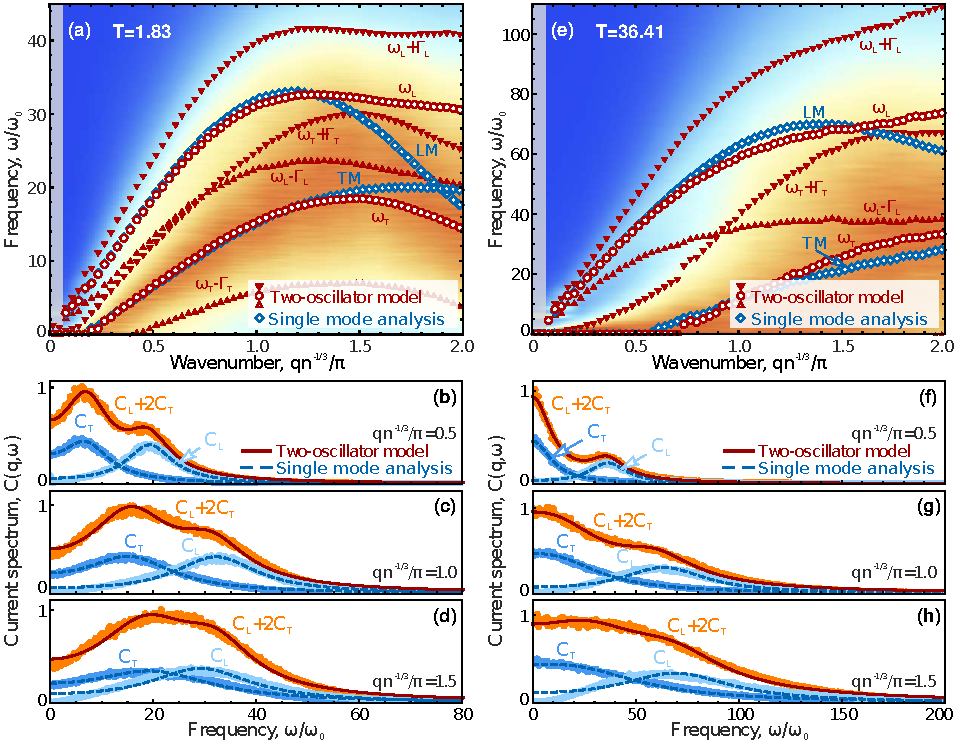
\includegraphics[width=0.7\textwidth]{Ris/CFS-Figure1.pdf}
\caption{Амплитуды и спектры возбуждений для трехмерной жидкости с потенциалом Леннарда-Джонса. }
\label{VelCurrent}
\end{center}
\end{figure}

Оба метода дают зависимости с разбросом значений частот $\omega_{L,T}(q)$ и коэффициентов взатухания $\Gamma_{L, T} (q)$. На рис. \ref{VelCurrent} можно увидеть результаты для Леннарда-Джонса при низких (a) - (d) и высоких (e) - (h)
температурах (T = 1.83 и 36.41 соответственно).




% (a) Спектр потока частиц $C(q, \omega)$ изображен в цветовом формате при $T = 1.83$ и $n = 1$, дисперсионные соотношения $\omega_{L, T}(q)$, полученные раздельной аппроксимацией, обозначены синими ромбами, соответствующими продольным и поперечным модам, а те, что получены совместной аппроксимацией, обозначены красными кругами. Треугольники
% соответствуют $\omega_{L, T} \pm \Gamma_{L, T}$. Зоны, обозначенные серым, соответствуют областям $qn^{-1/3} < 2\pi / L$. Панели (b) - (d) демонстрируют участки спектров потоков частиц при различных $qn^{-1/3}
% / \pi = 0.5, 1.0$ и $1.5$, полученных из моделирования (обозначены символами), и результаты аппроксимирования моделью 2DHO (5) и DHO (4) (показаны сплошной
% красной и пунктирными синими линиями соответственно). На панелях (e) - (h) аналогичные результаты, но полученные при T = 36.41 и n = 1.




На рис. \ref{VelCurrent}(а) представлены результаты $C (q, \omega)$ в цветовом формате. Синие ромбы соответствуют
дисперсионным соотношениям $\omega_{L, T} (q)$, рассчитанным путем раздельной аппроксимации продольной и поперечной мод. Результаты, полученные с помощью совместной аппроксимации,
показаны красными кругами для $\omega_{L, T} (q)$ и треугольниками для
$\omega_{L, T} (q) \pm \Gamma_{L, T}$. Результаты, полученные с помощью модели DHO, не изображены, поскольку они совпадают с теми, что уже показаны на рисунке. Профили $C (q, \omega)$, а также их продольные и поперечные составляющие $C_{L, T} (q, \omega)$ для различных значений волнового числа изображены на рис. \ref{VelCurrent}(b) - (d) символами, в то время как сплошные линии соответствуют результатам аппроксимации по формулам (\ref{DHO}) и (\ref{2DHO}).


Следует отметить, что оба подхода дают близкие
результаты, если полный спектр $C (q, \omega)$ имеет два хорошо выраженных максимума (на более низких и более высоких частотах, которые
обычно соответствуют продольным и поперечным модам), что обычно выполняется в первой псевдозоне Бриллюэна. Отклонение между дисперсионными соотношениями, полученными различными методами, растет с ростом температуры, как видно на рис. \ref{VelCurrent}(а) и \ref{VelCurrent}(е). Видно, что результаты,
полученные методами молекулярной динамики, хорошо согласуются с теоретическими подходами (\ref{DHO}) и (\ref{2DHO}).


При больших температурах и коротких
длинах волн, как показано на рис. \ref{VelCurrent}(h), результаты сильно искажаются, что связано с
изменением формы спектров на длинноволновом пределе. Если попереречные и продольные волны пересекаются, то модель DHO становится неприменимой (при $qn^{-1/3}/ \pi \simeq 1.9$). Смешивание мод и эффективное взаимодействие между ними сопровождается сильным перераспределением спектров и гибридизацией \cite{101103, 112101}.






\section{Анализ спектров в комплексной (пылевой) плазме}



%Теория, моделирование и эксперименты наглядно демонстрируют наличие антикроссинга мод, которое сопровождается гибридизацией и сильным перераспределением спектров возбуждения.


Для анализа скрещивания мод в сильно связанных жидкостях с потенциалом Юкавы было проведено моделирование МД для квазидвумерной жидкости при  $\varepsilon = e^2 Z^2 /4\pi \varepsilon_0 \lambda_D = 874 ~\text{эВ}$, где $Z = 1.25 \times 10^4$ - зарядовое число, $\lambda_D  = 260~ \text{нм}$ - длина экранировки Дебая. 

Система состояла из $N = 10^4$ частиц с массами, равными $m = 6.1 \times 10^{-10}~ \text{гр}$, помещенными в кубическую область с периодическими граничными условиями со сторонами $L = 30.5~ \text{м}$. Частицы находились в параболической потенциальной яме $U(z)  = 0.5 m \Omega_z^2 z^2$, где $\Omega_z^2 = 25 ~\text{Гц}$ - частота поперечных колебаний частиц  в длинноволновом пределе. 



Радиус отсечки был взят равным $r_c = 2.29~ \text{мм}$, что примерно соответствовало 7.5 межчастичных расстояний. Моделирование проводилось в термостате Ланжевена с $T = 18~ \text{эВ}$, скоростью затухания $\nu = 1.8 ~\text{с}^{-1}$ и шагом по времени $\Delta t = 38~ \text{нс}$. На начальном этапе была задана квадратная решетка в плоскости $z = 0$ с плотностью $\rho = 1/V_0 = N/L^2 = 10.75~ \text{мм}^{-2}$ при температуре $T = 26.9~ \text{эВ}$ (которая соответствует распределению Максвелла). Первые $10^{6}$ шагов система находилась в состоянии равновесия, затем следующие $10^6$ шагов были использованы для анализа спектров флуктуаций.




На рис. \ref{PlasmaSp} изображены спектры элементарных возбуждений для квазидвумерных жидкостей с потенциалом Юкавы. 

\begin{figure}[htbp]
    \begin{center}
    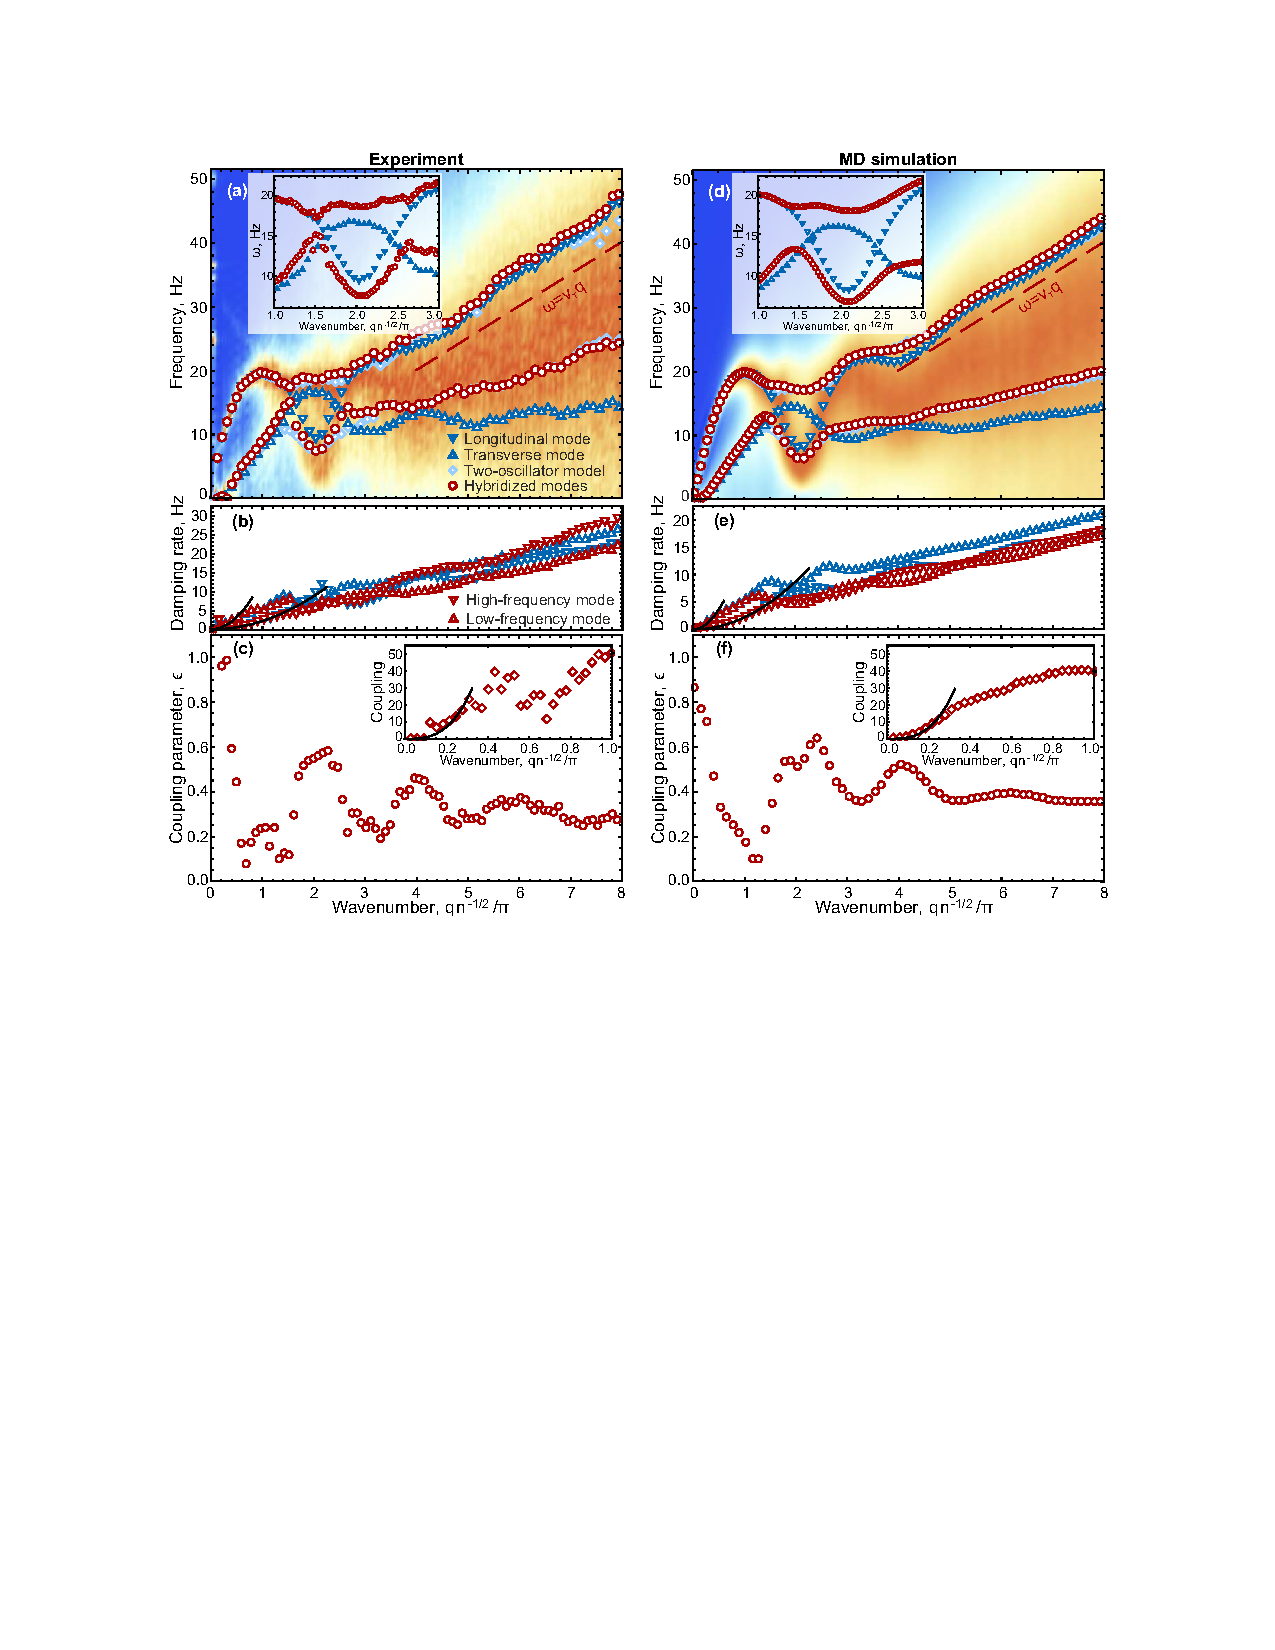
\includegraphics[width=0.7\textwidth]{Ris/Plasma_SP_3.pdf}
    \caption{Амплитуды и спектры возбуждений для квазидвумерной жидкости с потенциалом Юкавы. }
    \label{PlasmaSp}
    \end{center}
\end{figure}

На (a) - (c) изображены спектры, скорости затухания и параметры связи между продольными и поперечными возбуждениями, полученные в ходе эксперимента, а на панелях (d) - (f) - результаты, полученные методом МД.

Видно, что данные, полученные в ходе эксперимента, согласуются с результатами МД. Наблюдаемые различия обусловлены лучшей статистикой МД и более сложными взаимодействиями в эксперименте из-за плазменных вейков. Антикроссинг мод наблюдается при $q^{-1/2} \pi^{-1} \approx 1.6$ или $2.4$ (в диапазоне волновых чисел между коллективной и одночастичной динамикой), где две пересекающиеся моды (показанные синими треугольниками) отталкиваются друг от друга. В результате антикроссинга наблюдается высокочастотные и низкочастотные моды гибридизированных возбуждений, представленные красными кругами на рис.  \ref{PlasmaSp}(a) и  \ref{PlasmaSp}(d) вместо продольных и поперечных возбуждений, показанных синими треугольниками.

\begin{figure}[htbp]
\begin{center}
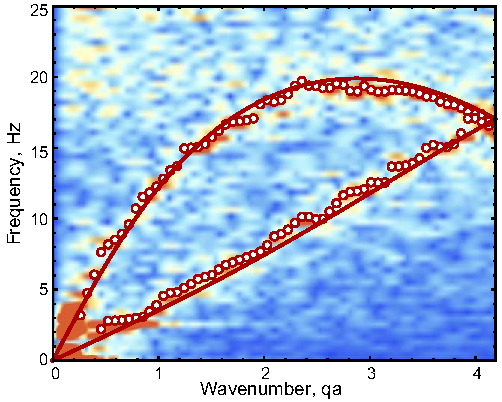
\includegraphics[width=0.6\textwidth]{Ris/Plasma_SP_1.pdf}
\caption{Спектры возбуждений для кристалла с потенциалом Юкавы.}
\label{PlasmaSp2}
\end{center}
\end{figure}

В жидкостях возбуждения сильно демпфированы и поэтому продольная и поперечная составляющие амплитуды $C(q, \omega) = C_{\parallel}(q, \omega) + C_{\perp}(q, \omega)$, показанные на рис.  \ref{PlasmaSp}(a) и  \ref{PlasmaSp}(d) оказываются размытыми в плоскости $(q,\omega)$.  Скорости затухания представлены на рис.  \ref{PlasmaSp}(b) и \ref{PlasmaSp}(e). Сплошные черные линии показывают для эксперимента и моделирования диффузионное затухание $\Gamma_{\parallel, \perp} \sim q^2$ на небольших $q$. Безразмерный параметр связи $\varepsilon$ показан на рис.  \ref{PlasmaSp}(c) и \ref{PlasmaSp}(f) для эксперимента и моделирования МД. Сплошная черная линия на (c), (f) -  это результаты аппроксимации $\varepsilon \Omega_{\parallel, \perp} \sim q^3$. Данное соотношение получается из того, что при малых $q$ $ \Omega_{\parallel} \approx   \omega_{\perp} \sim q$, а $\Omega_{\perp} \approx   \omega_{\parallel} \sim q^2$.



Фононный спектр в комплексной (пылевой) плазме изображен на рис. \ref{PlasmaSp2}: амплитуды показаны в цветовом формате; красные символы показывают дисперсионные соотношения $\omega_{\parallel, \perp}(q)$ для продольных и поперечных колебаний, полученные путем аппроксимации экспериментально полученных значений $C(q, \omega)$ моделью затухающего гармонического осциллятора. Сплошная красная линия соответствует теоретическим дисперсионным соотношениям для кристаллов с потенциалом Юкавы.


\section{Выводы}

Метод, основанный на модели 2DHO, пригоден для анализа возбуждений в
 в двумерных и трехмерных жидкостях с различными потенциалами взаимодействия. Однако в длинноволновом пределе наблюдается возврат к режиму индивидуальной динамики частиц, при котором
продольные и поперечные спектры потока определяются распределениями Максвелла по скоростям.

Полученные результаты могут быть применены для анализа возбуждений в жидкой комплексной (пылевой) плазме.
Так же с помощью данного подхода можно детального анализировать возбуждения в жидких средах различной природы, от
простых жидкостей и благородных газов до жидких металлов, молекулярных и сложных жидкостей. Смешивание мод в сильно связанных жидкостях приводит к эффективному взаимодействию между продольными и поперечными возбуждениями, что приводит к антикроссингу мод. Детальный анализ возбуждений открывает захватывающие перспективы для установления  соотношений между индивидуальной, коллективной динамиками и
термодинамикой жидкостей. 

\newpage

\newpage
\begin{center}
\textbf{ГЛАВА 3}\\
\textbf{ДИФФУЗИЯ ОТ ТРОЙНОЙ ДО КРИТИЧЕСКОЙ ТОЧКИ}
\end{center}
\refstepcounter{chapter}


% \section*{}
\addcontentsline{toc}{chapter}{ГЛАВА 3. Диффузия от тройной до критической точки}


\section{Изучение диффузии методами молекулярной динамики}\label{C3_1}

Имея координаты всех частиц в системе, можно пронаблюдать за перемещением каждой частицей в отдельности и оценить коэффициент диффузии и другие параметры переноса в данной системе.

На рисунке \ref{risTreck} изображены траектории частиц в исследуемой системе на примере потенциала Леннарда - Джонса при различной температуре.  Для демонстрации динамики системы были взяты первые 10 кадров, используемые в статистике, описанной в разделе \ref{C2_2}, с шагом по времени между кадрами равными $0.5\tau$. Траектории раскрашены в зависимости от перемещения частицы за 10 кадров наблюдения, частицам, практически не поменявшим свое расположение соответствует темно-синий цвет. В данном случае наиболее оптимальным было считать максимальным перемещением $3\sigma$, где $\sigma$ - безразмерная единица измерения длинны в моделировании, равная единице.

Как можно заметить, частицы, распознанные как конденсат в разделе \ref{C2_2}, демонстрируют меньшие длинны траектории, чем газ, что свидетельствует о достаточно хорошей точности распознавания фаз, описанной в разделе \ref{C2_1}. 

\begin{figure}[h]
\begin{center}
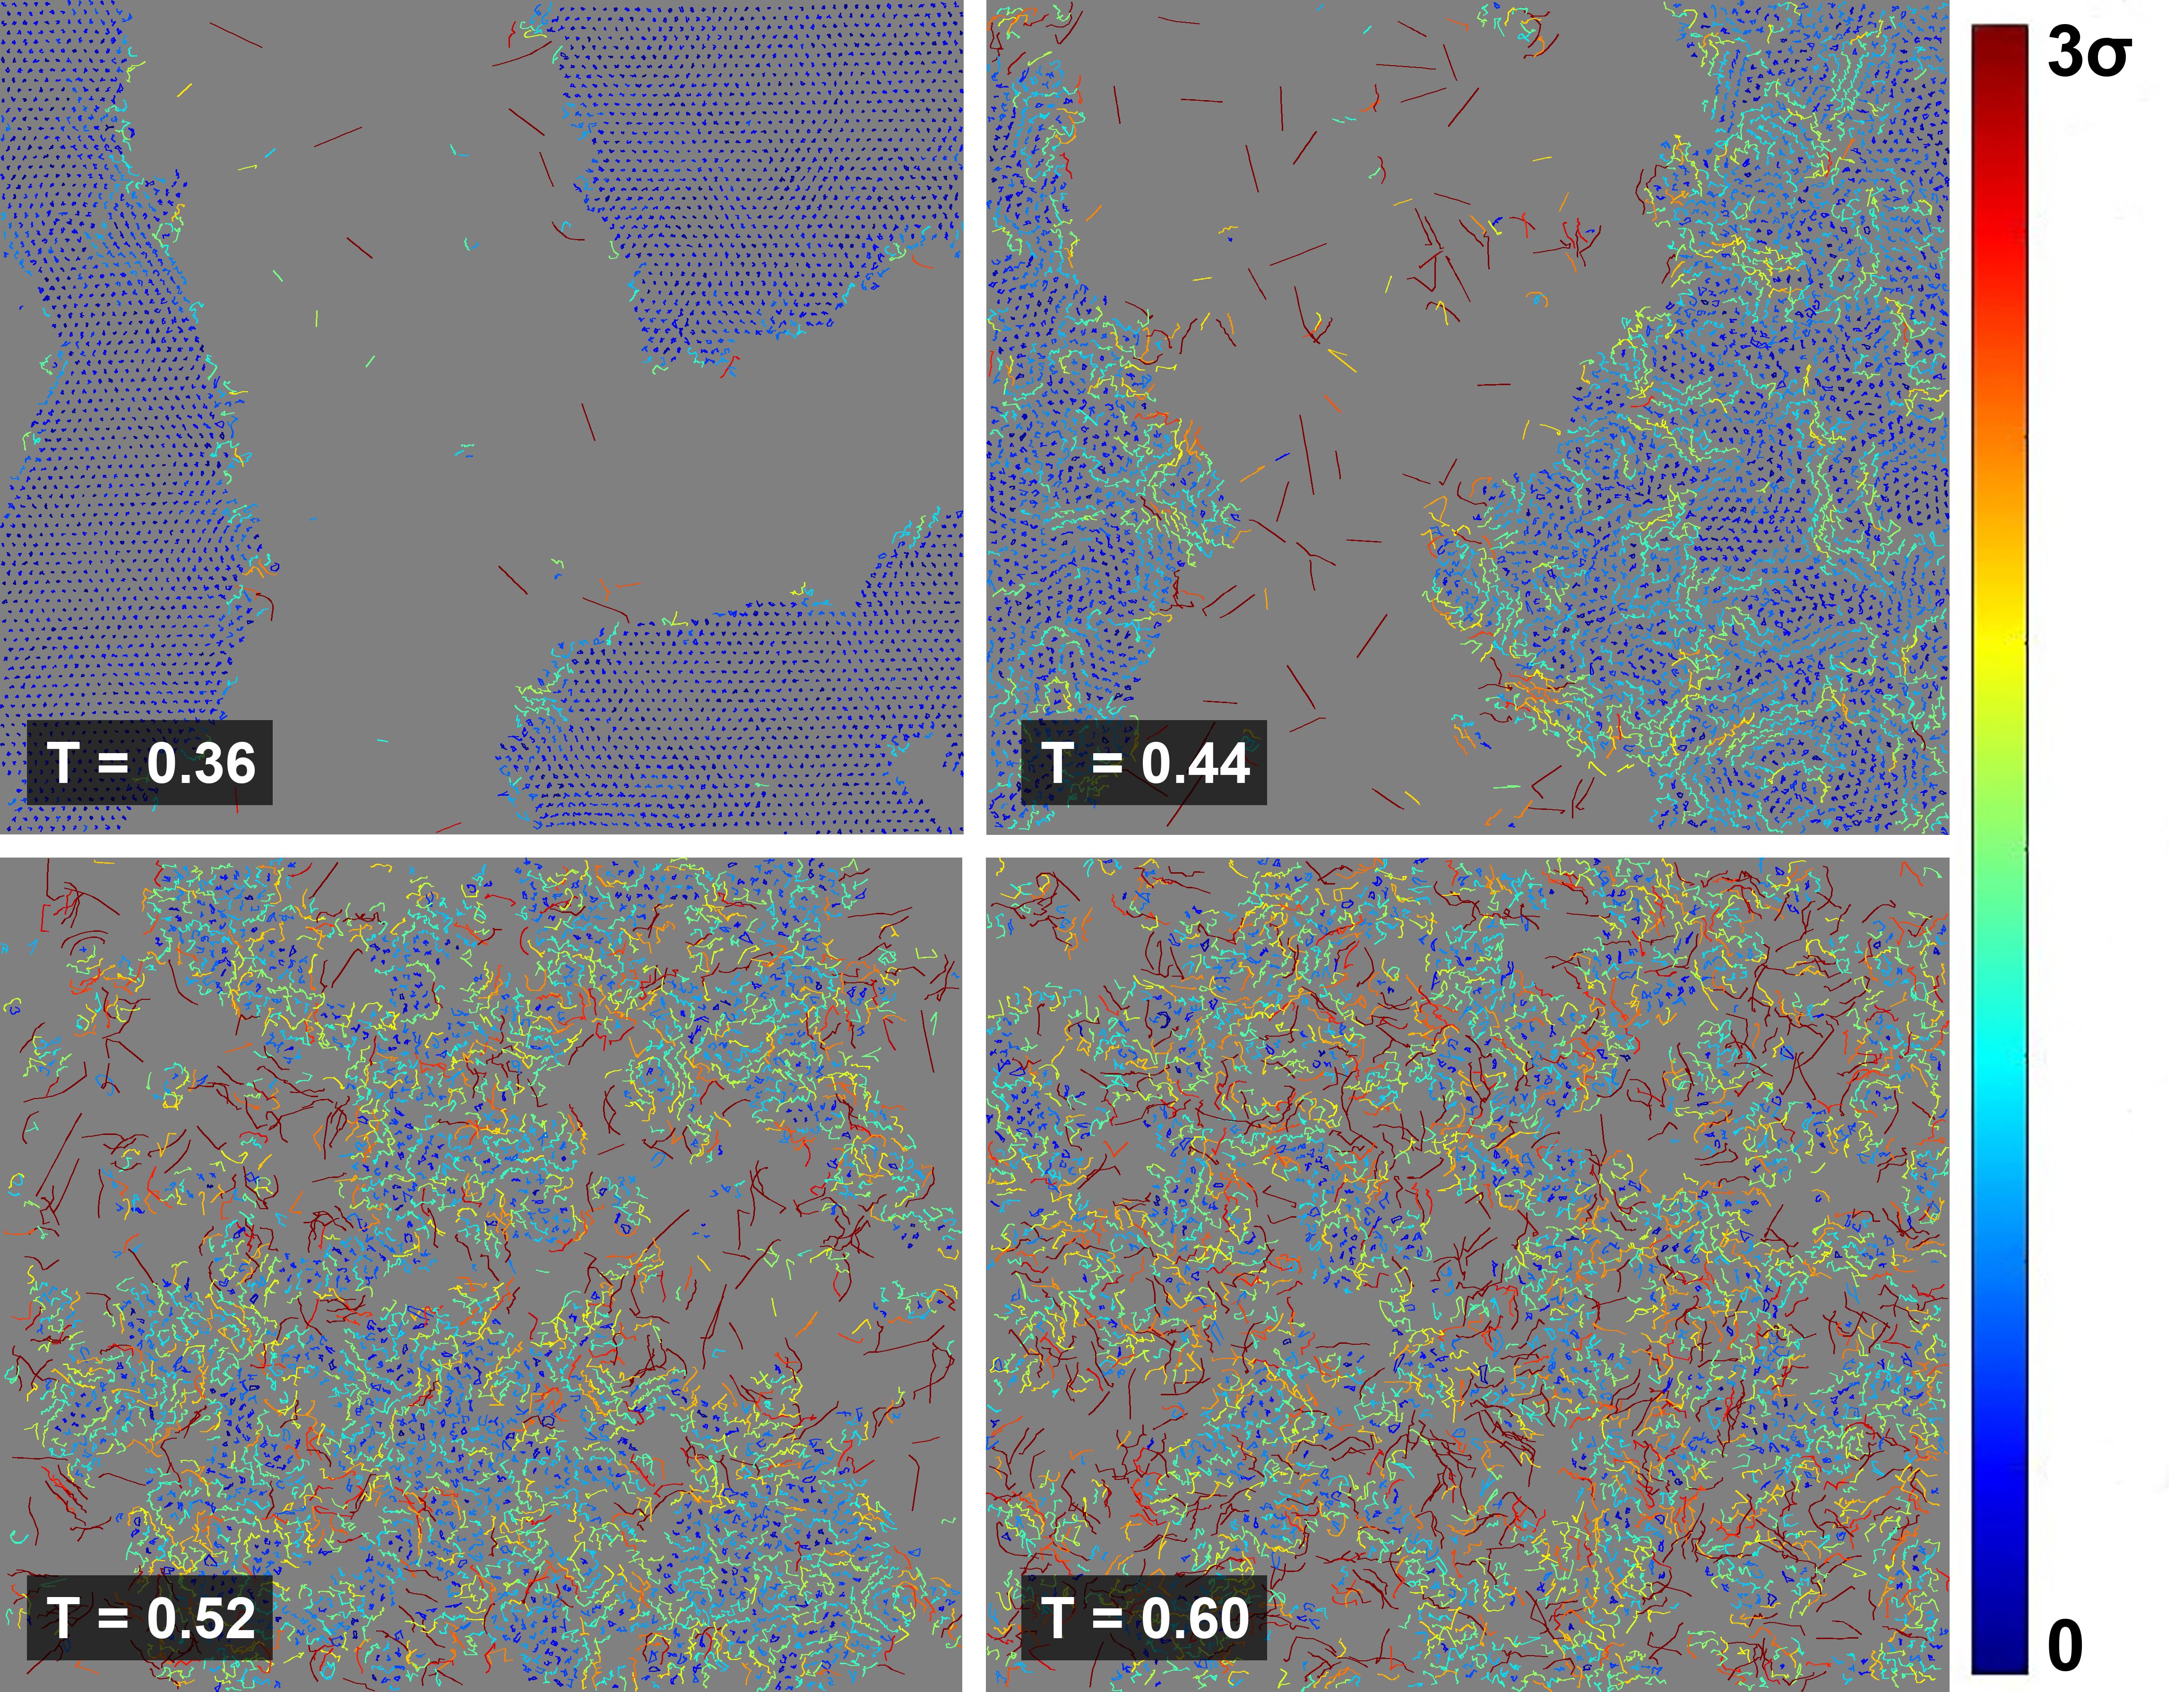
\includegraphics[width=0.7\textwidth]{Diffusion}
\caption{Смещение частиц от начального положения за 10 кадров моделирования. Цветом показана величина смещения в $\sigma$ (единица измерения длинны). Наиболее подвижным частицам соответствует темно-красный цвет траектории.}
\label{risTreck}
\end{center}
\end{figure}

Количество частиц на кадре в общем случае может быть не одинаковым. В реальных экспериментах с коллоидными суспензиями это обусловлено смещением частиц за пределы кадра, или потерей частицы на кадре из-за неидеальности распознавания объектов на изображении используемым методом. В случае моделирования причинами непостоянства количества частиц могут быть смещение частицы за пределы исследуемой области, либо отсева частиц с бесконечными гранями ячейки вороного, расположенной на периферии, для которой не удается определить не соседей, ни площади. Такие частицы не участвуют в статистике ни расчета термодинамических параметров во второй главе, ни в расчете параметров переноса. 

Зная смещения всех частиц от их изначального положения в системе, с $t = 0$, можно рассчитать среднеквадратичное смещение частиц с помощью уравнения:
\begin{equation}
    \sigma^2(t) = \sum\limits_{\alpha = 1}^{N(t)} (r_{\alpha}(t) - r_{\alpha}(0))^2 / N(t),
    \label{eqRMS}
\end{equation}
где $\sigma^2(t)$ - среднеквадратичное смещение частиц, $N(t)$ - количество частиц в данный момент времени в кадре, $r_{\alpha}(t)$ - положение частицы в момент времени $t$, $r_{\alpha}(0)$ - положение частицы в начальный момент времени $t = 0$.

\begin{figure}[h]
\begin{center}
\begin{minipage}[h]{0.45\linewidth}
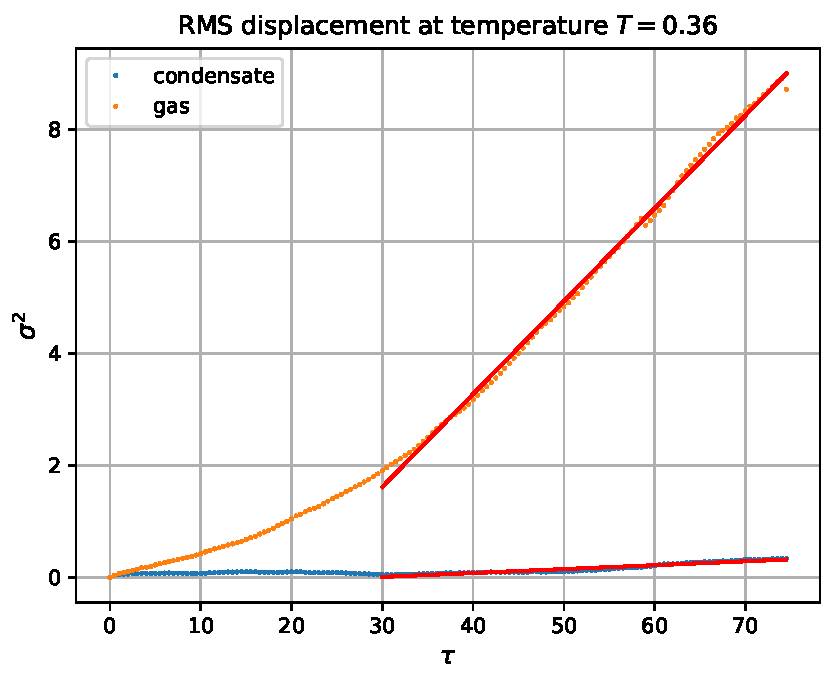
\includegraphics[width=\textwidth, keepaspectratio]{diffusion_fit_0.36}
\end{minipage}
%\hfill
\begin{minipage}[h]{0.45\linewidth}
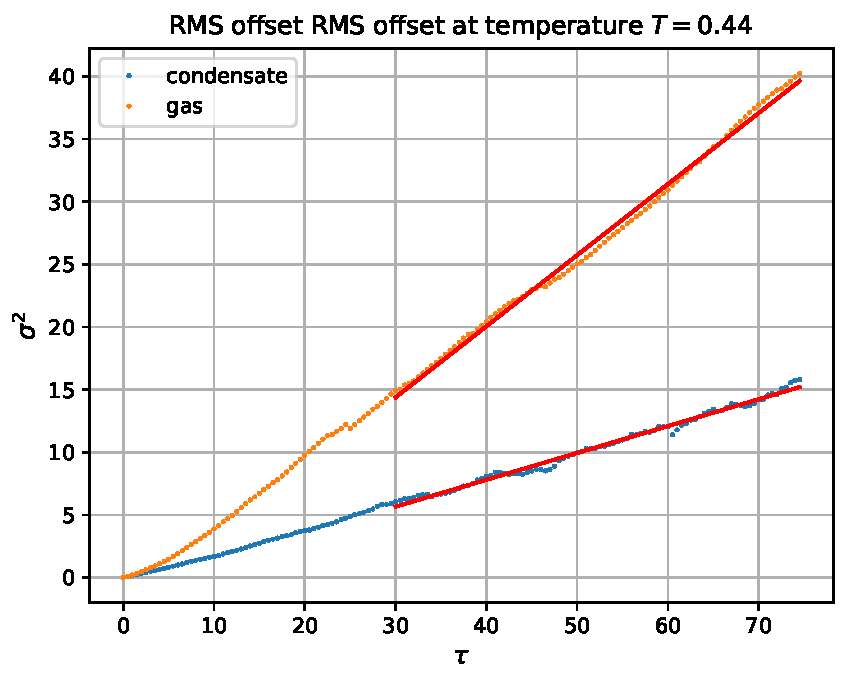
\includegraphics[width=\textwidth, keepaspectratio]{diffusion_fit_0.44}
\end{minipage}

\begin{minipage}[h]{0.45\linewidth}
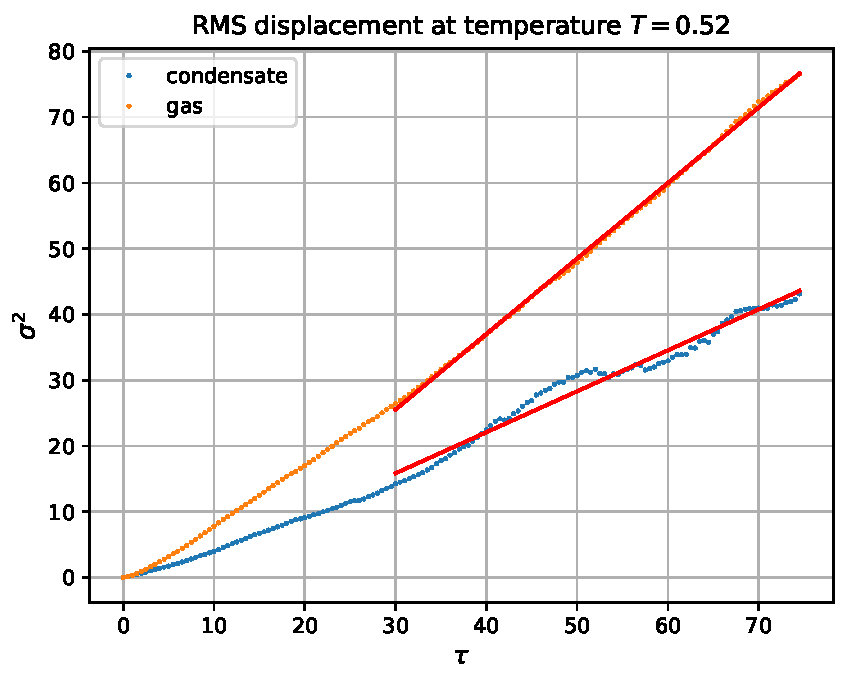
\includegraphics[width=\textwidth, keepaspectratio]{diffusion_fit_0.52}
\end{minipage}
%\hfill
\begin{minipage}[h]{0.45\linewidth}
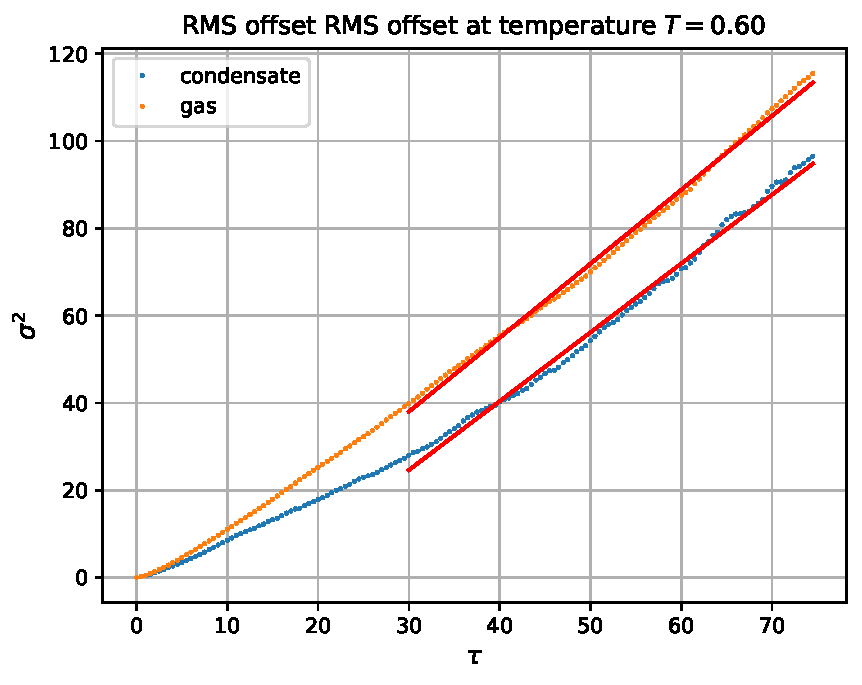
\includegraphics[width=\textwidth, keepaspectratio]{diffusion_fit_0.60}
\end{minipage}
\caption{Временная зависимость среднеквадратичного смещения частиц для различных температур на примере потенциала Леннарда-Джонса. Синим цветом обозначено среднеквадратичное смещение конденсированных частиц,  а оранжевым - всех частиц в исследуемой системе.}
\label{risRMS}
\end{center}
\end{figure}

График зависимости среднеквадратичного смещения для подсистем конденсированных частиц и всех (все частицы в системе, включая газовые и конденсат) от безразмерного времени для различных температур изображен на рисунке \ref{risRMS}.

Так как для двумерной системы верно равенство $\sigma^2(t) = 4Dt$, то коэффициент диффузии выражается следующей формулой:
\begin{equation}
    D = \frac{\sigma^2(t)}{4t},
    \label{eqD}
\end{equation}
где $D$ - коэффициент диффузии в веществе.

Его можно получить путем аппроксимации среднеквадратичного смещения функцией $\sigma^2(t) = 4Dt + a$, где $a$ - подгоночный коэффициент. Подгоночный коэффициент $a$ появляется в следствие того, что аппроксимация производится начиная не с 0 по времени, а с некоторого значения, когда функция становится линейной. Данный эффект хорошо наблюдается при $T = 0.36$ на рисунке \ref{risRMS}. экспериментально установлено, что для данных экспериментов достаточно использовать последние $60\%$ точек, для правильной аппроксимации. 
На рисунке \ref{risRMS} она показана сплошной красной линией, которая аппроксимирует среднеквадратичное смещение с достаточно хорошей точностью.

\begin{figure}[h]
\begin{center}
\begin{minipage}[h]{0.45\linewidth}
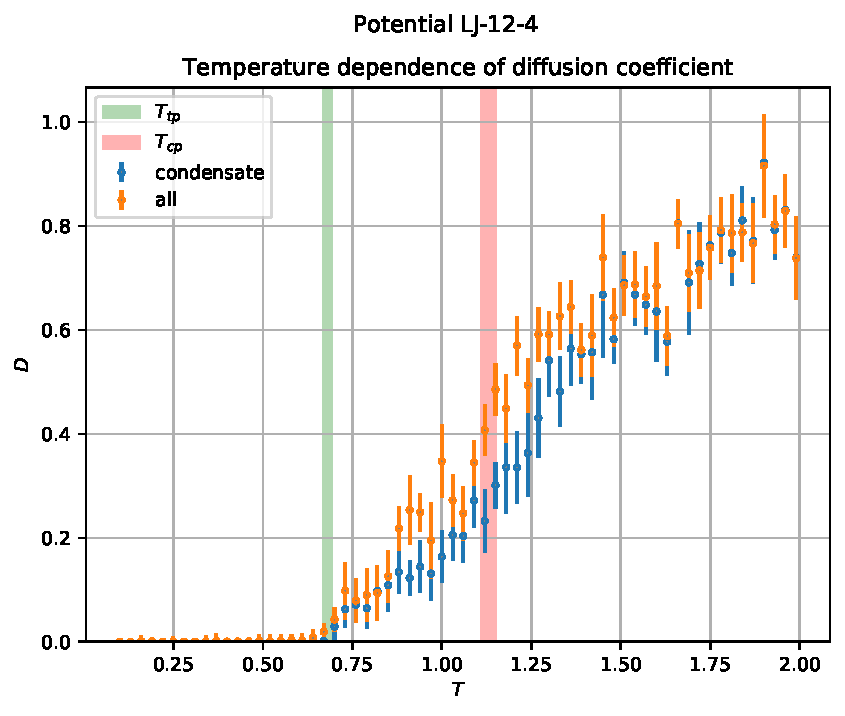
\includegraphics[width=\textwidth, keepaspectratio]{plot_diffusion_Potential LJ-12-4_1}
\end{minipage}
\begin{minipage}[h]{0.45\linewidth}
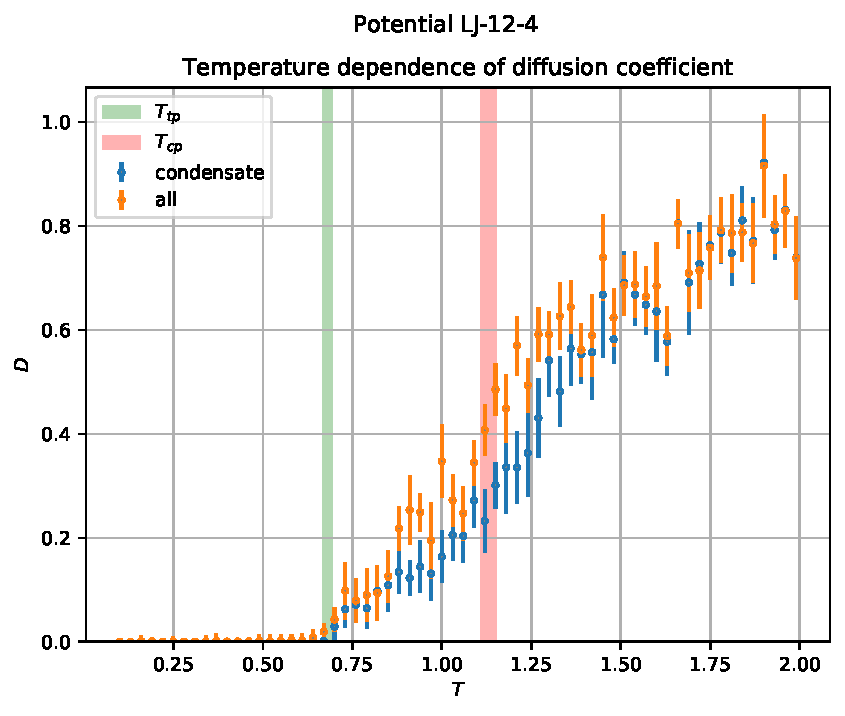
\includegraphics[width=\textwidth, keepaspectratio]{plot_diffusion_Potential LJ-12-4_1}
\end{minipage}
\begin{minipage}[h]{0.45\linewidth}
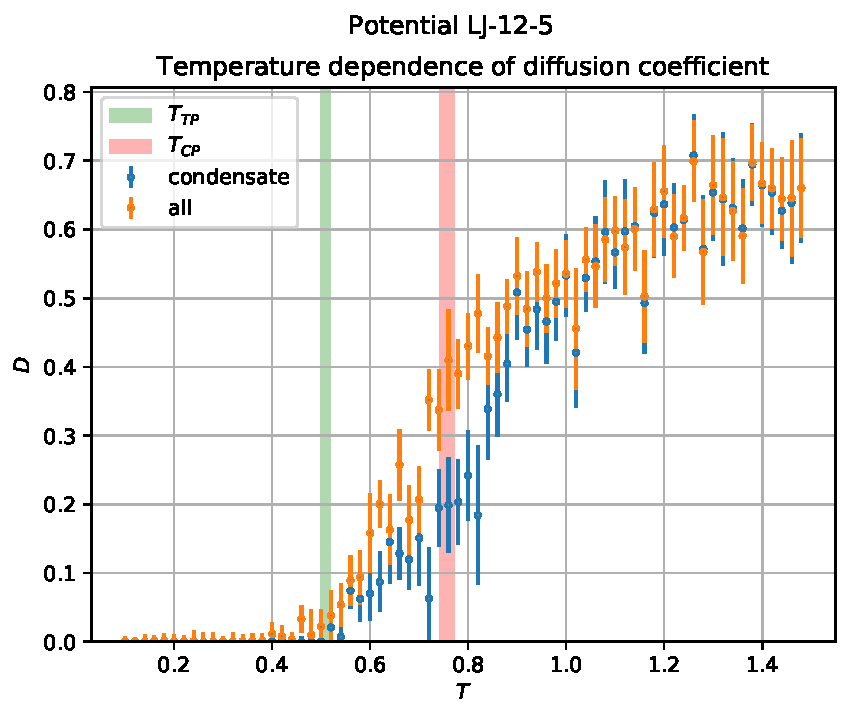
\includegraphics[width=\textwidth, keepaspectratio]{plot_diffusion_Potential LJ-12-5_1}
\end{minipage}
\begin{minipage}[h]{0.45\linewidth}
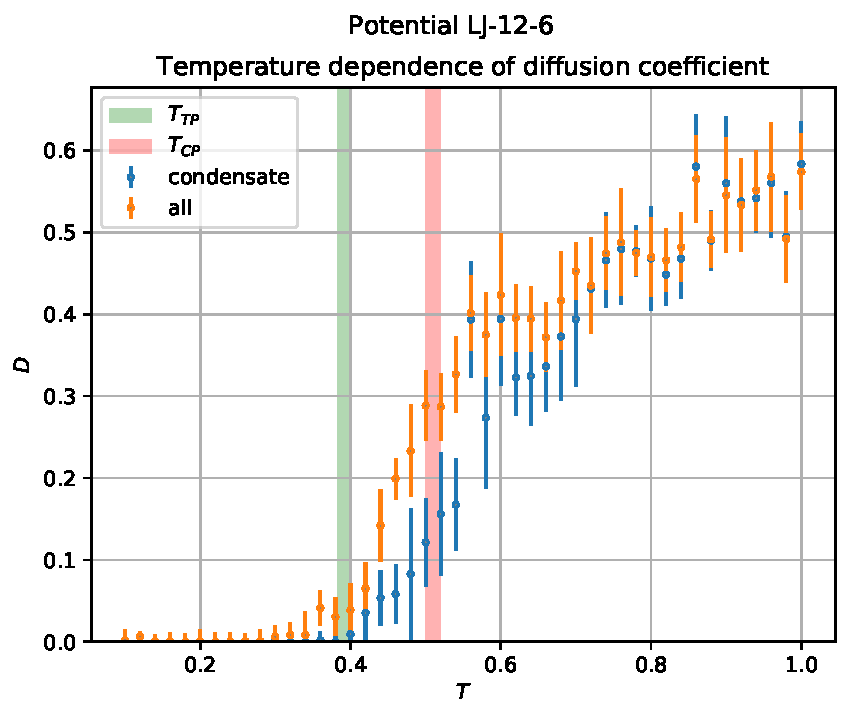
\includegraphics[width=\textwidth, keepaspectratio]{plot_diffusion_Potential LJ-12-6_1}
\end{minipage}
\caption{Температурная зависимость коэффициента диффузии для различных потенциалов взаимодействия. Не доделана!}
\label{risD}
\end{center}
\end{figure}

Проводя данные вычисления для различных температур, можно установить температурную зависимость коэффициента диффузии для различных потенциалов взаимодействия, изображенную на рисунке \ref{risD}.

Полученные результаты хорошо согласуются с экспериментом, например в $LJ12-6$ температура плавления $T_{TP} = 0.405$, что соответствует температуре, при которой значение коэффициента диффузии начинает расти.

Коэффициент диффузии, рассчитанный таким образом, может быть использован для определения тройной точки, так как однозначно при различных потенциалах показывает резкий рост смещения частиц относительно своих изначальных положений, что характерно при плавлении веществ.

\begin{figure}[h]
\begin{center}
\begin{minipage}[h]{0.45\linewidth}
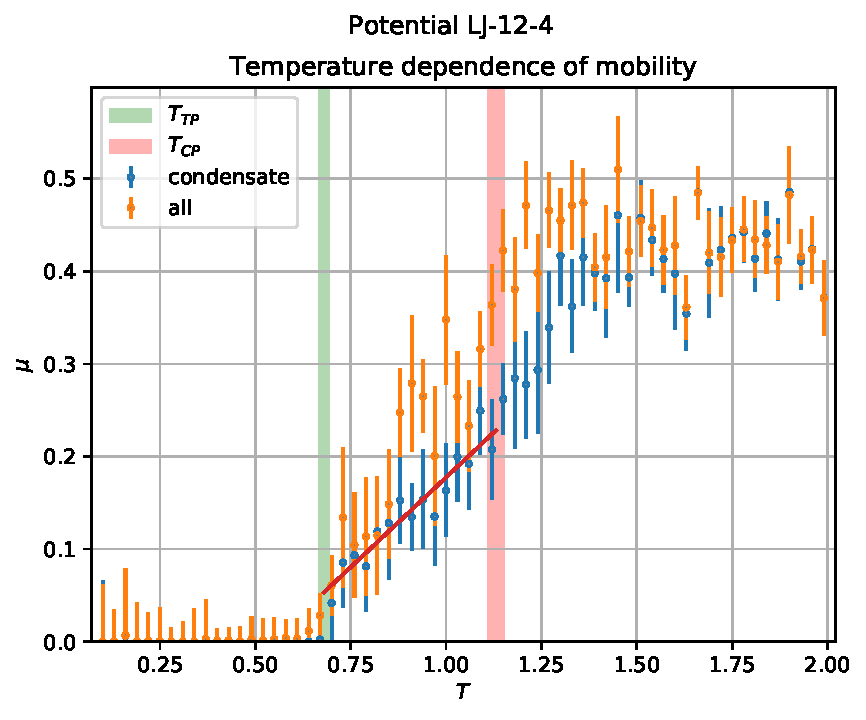
\includegraphics[width=\textwidth, keepaspectratio]{plot_mobility_Potential LJ-12-4_1}
\end{minipage}
%\hfill
\begin{minipage}[h]{0.45\linewidth}
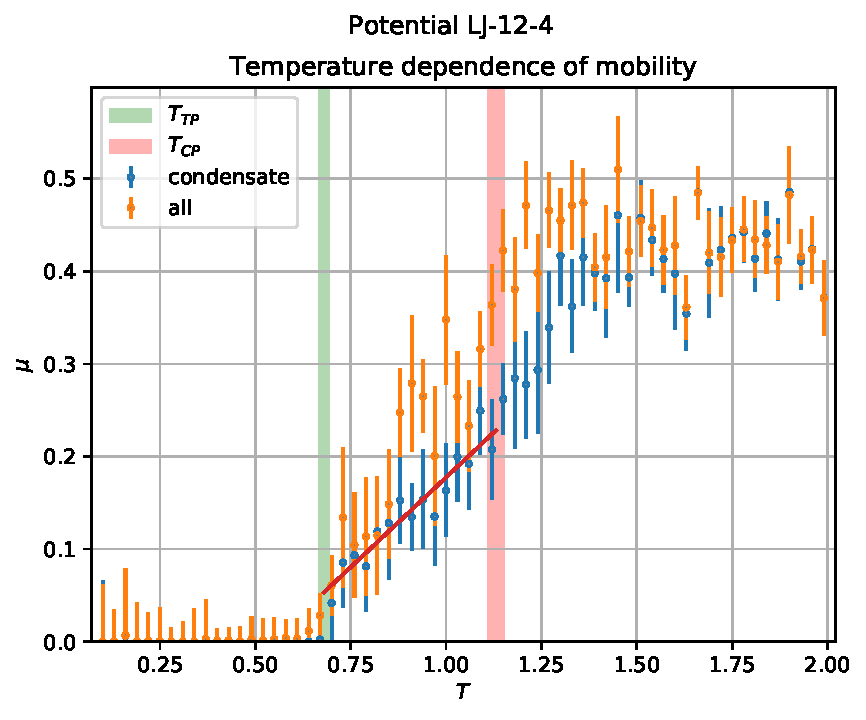
\includegraphics[width=\textwidth, keepaspectratio]{plot_mobility_Potential LJ-12-4_1}
\end{minipage}
\begin{minipage}[h]{0.45\linewidth}
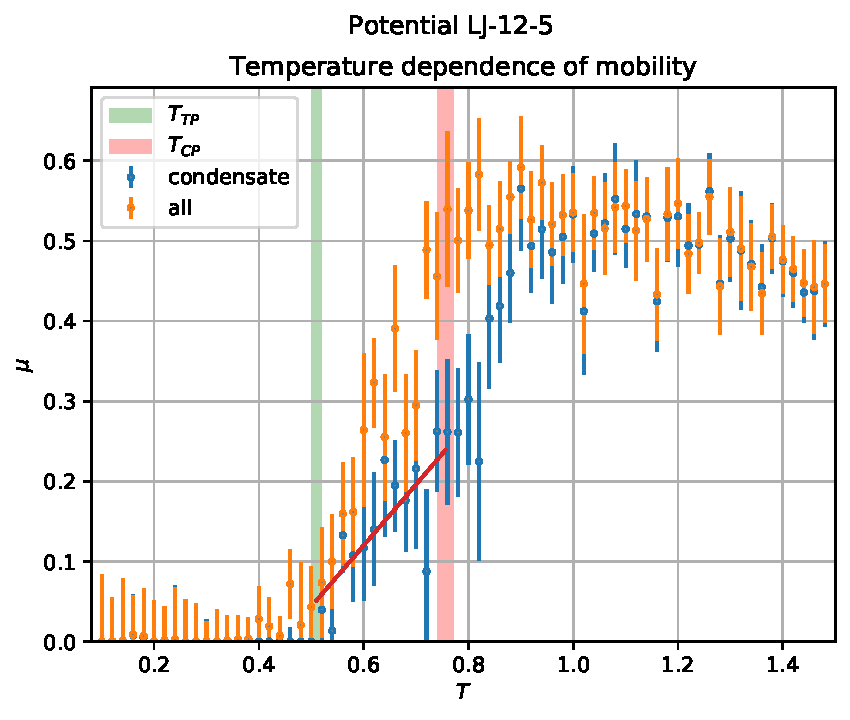
\includegraphics[width=\textwidth, keepaspectratio]{plot_mobility_Potential LJ-12-5_1}
\end{minipage}
%\hfill
\begin{minipage}[h]{0.45\linewidth}
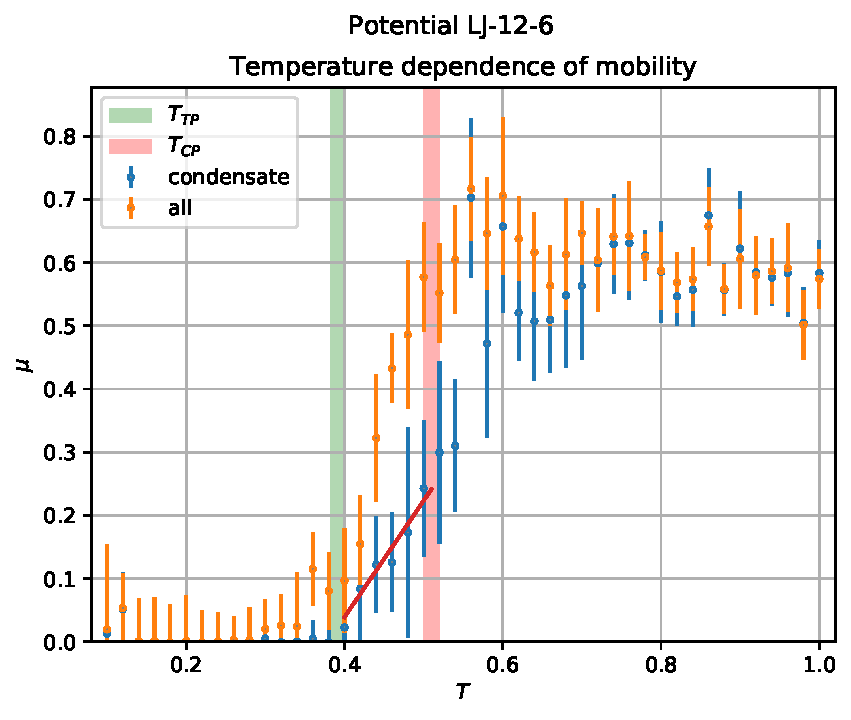
\includegraphics[width=\textwidth, keepaspectratio]{plot_mobility_Potential LJ-12-6_1}
\end{minipage}
\caption{Температурная зависимость подвижности для различных потенциалов взаимодействия. Не доделана!}
\label{risMuDiff}
\end{center}
\end{figure}

Кроме диффузии мы можем вычислить подвижность частиц в системе, которая определяется следующим образом:
\begin{equation}
    \mu  = \frac{D}{T},
    \label{eqMuDiff}
\end{equation}
где $\mu$ - подвижность частиц.

Зависимость подвижности частиц от температуры представлена на рисунке \ref{risMuDiff}.
Как можно заметить, данная зависимость практически линейна в промежутке от тройной до критической точки. Аппроксимация подвижности частиц в пределах жидкой фазы позволяет выяснить температурное влияние на изменение подвижности, в зависимости от дальнодействия притяжения.

\begin{figure}[h]
\begin{center}
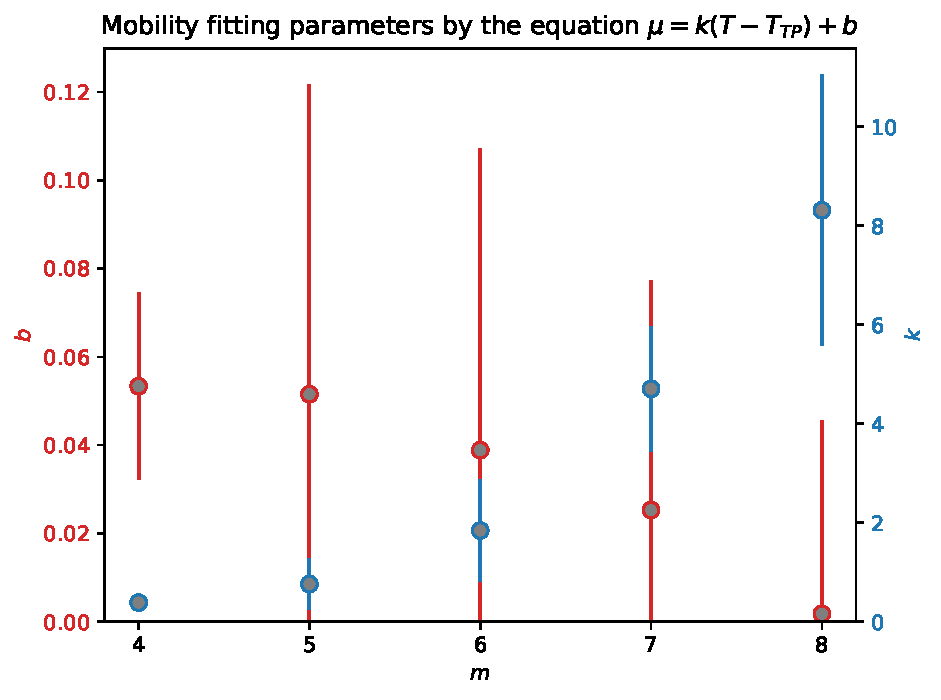
\includegraphics[width=\textwidth]{mobility_fitting_factors}
\caption{График зависимости параметров аппроксимации подвижности от тройной до критической точки линейной функцией.}
\label{risDmu}
\end{center}
\end{figure}

На рисунке \ref{risDmu} представлена зависимость параметров аппроксимации мобильности от тройной до критической точки линейной функцией. Физический смыл у данных коэффициентов следующий, $b$ - значение подвижности частиц в тройной точке, а $k$ - производная значения подвижности по температуре. 

Анализируя зависимость подвижности в тройной точке, можно предположить, что ее уменьшение с уменьшением дальнодействия связано с уменьшением ширины потенциальной ямы, в которой находится частица. В то же время отклик системы на повышение температуры, которым является параметр $k$, повышается. Это может быть связано с уменьшением потенциальной ямы, в которой находится частицы, что позволяет ей легче передвигаться и из нее выходить.

В случае дальнейшего уменьшения дальнодействия в системе, можно будет наблюдать переход вещества в состояние геля, для которого характерно очень сильное влияние температуры на подвижность частиц.


\section{Связь термодинамических параметров и параметров переноса вещества}\label{C3_2}

В попытках выяснить зависимость параметров переноса вещества от его термодинамических параметров, были построены зависимости мобильности от сжимаемости и диффузии (рисунки \ref{risMuBeta}, \ref{risDBeta}), а так же зависимость скорости звука от мобильности (рисунок \ref{risCMu}).

\begin{figure}[h]
\begin{center}
\begin{minipage}[h]{0.45\linewidth}
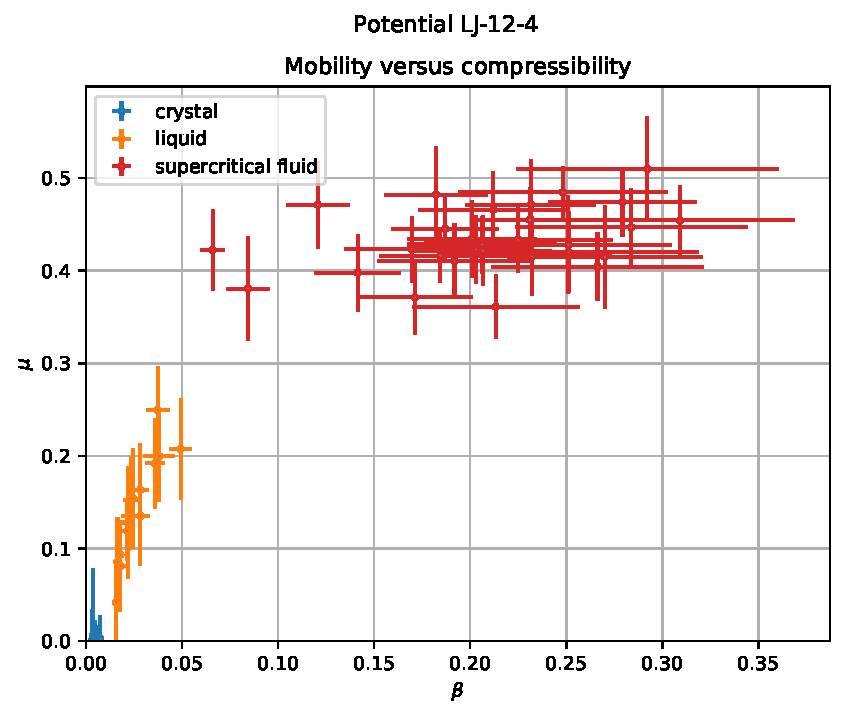
\includegraphics[width=\textwidth, keepaspectratio]{plot_compress_mobility_Potential LJ-12-4_1}
\end{minipage}
%\hfill
\begin{minipage}[h]{0.45\linewidth}
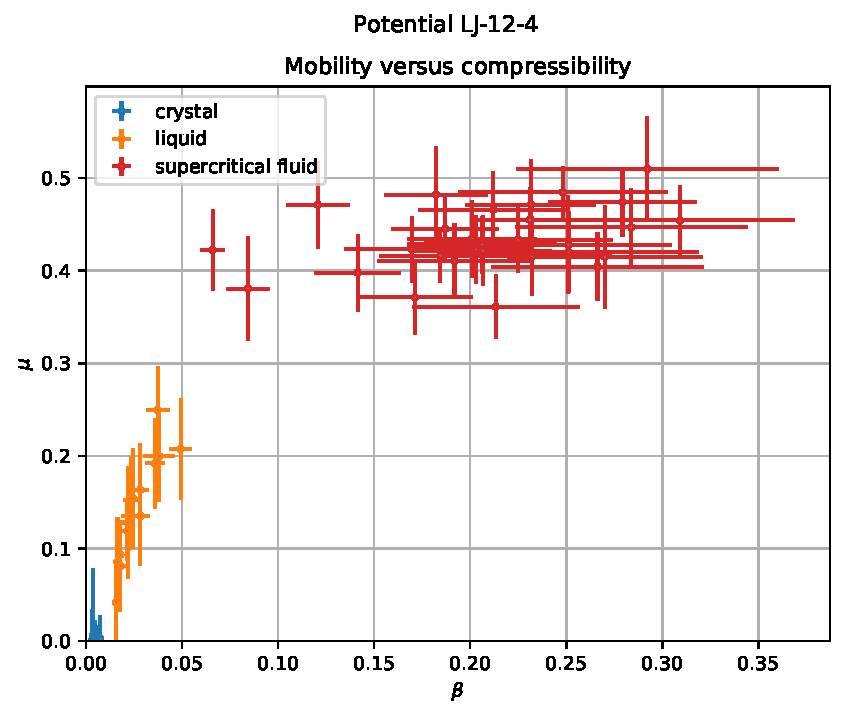
\includegraphics[width=\textwidth, keepaspectratio]{plot_compress_mobility_Potential LJ-12-4_1}
\end{minipage}

\begin{minipage}[h]{0.45\linewidth}
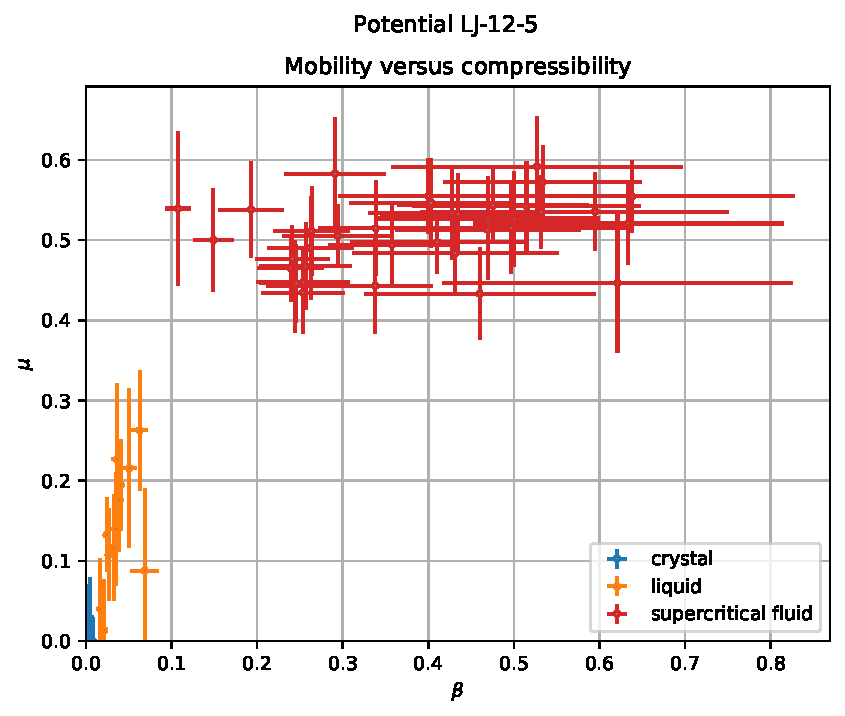
\includegraphics[width=\textwidth, keepaspectratio]{plot_compress_mobility_Potential LJ-12-5_1}
\end{minipage}
%\hfill
\begin{minipage}[h]{0.45\linewidth}
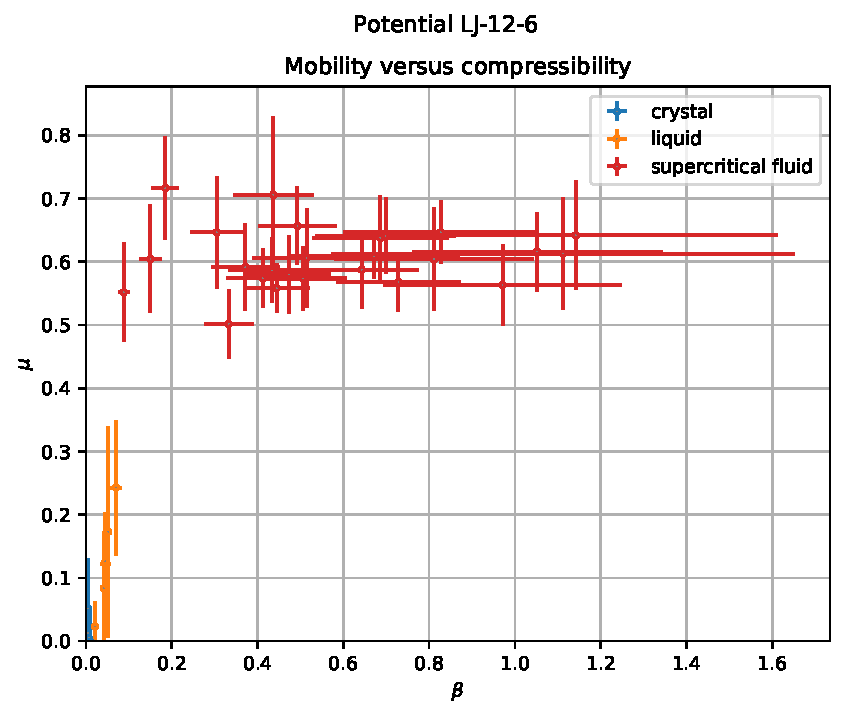
\includegraphics[width=\textwidth, keepaspectratio]{plot_compress_mobility_Potential LJ-12-6_1}
\end{minipage}
\caption{Зависимость мобильности от сжимаемости. Не доделана!}
\label{risMuBeta}
\end{center}
\end{figure}


\begin{figure}[h]
\begin{center}
\begin{minipage}[h]{0.45\linewidth}
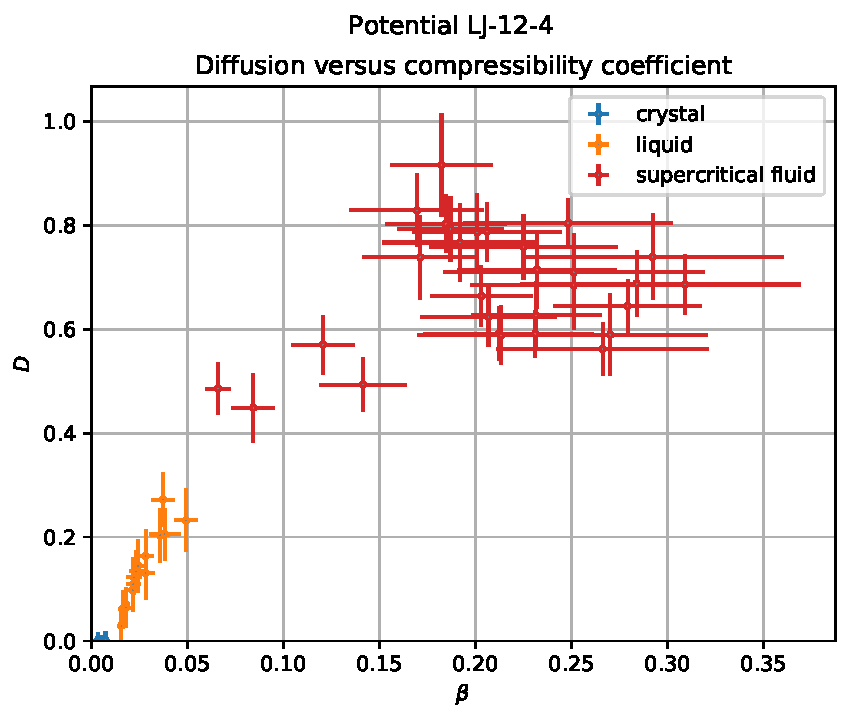
\includegraphics[width=\textwidth, keepaspectratio]{plot_diffusion_compress_Potential LJ-12-4_1}
\end{minipage}
%\hfill
\begin{minipage}[h]{0.45\linewidth}
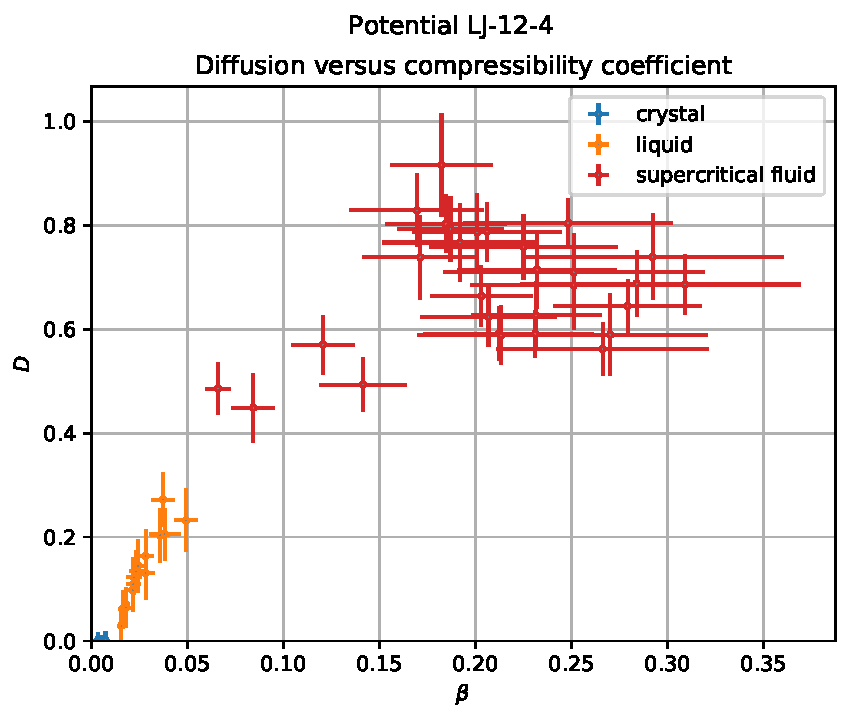
\includegraphics[width=\textwidth, keepaspectratio]{plot_diffusion_compress_Potential LJ-12-4_1}
\end{minipage}

\begin{minipage}[h]{0.45\linewidth}
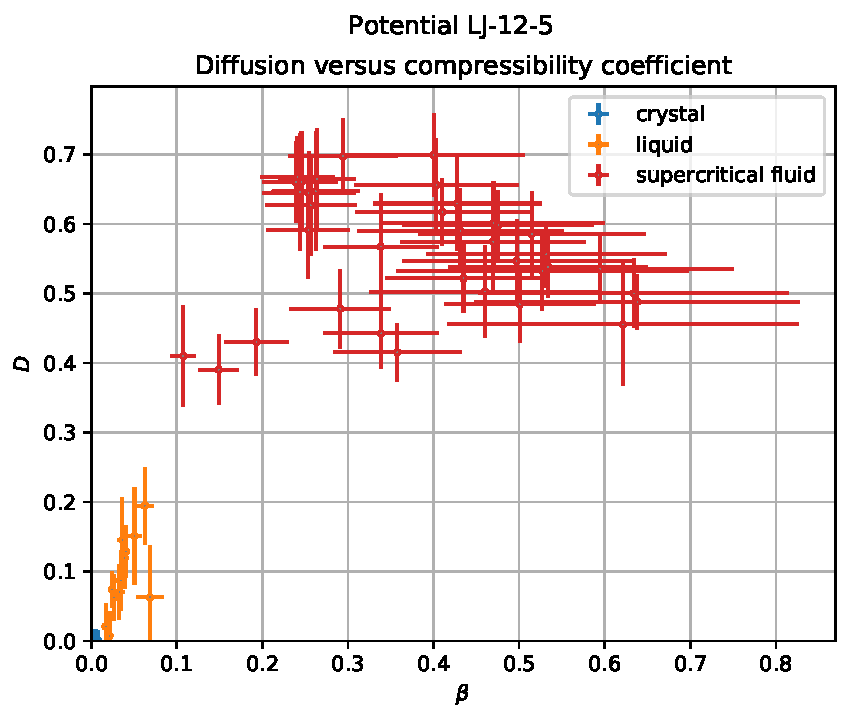
\includegraphics[width=\textwidth, keepaspectratio]{plot_diffusion_compress_Potential LJ-12-5_1}
\end{minipage}
%\hfill
\begin{minipage}[h]{0.45\linewidth}
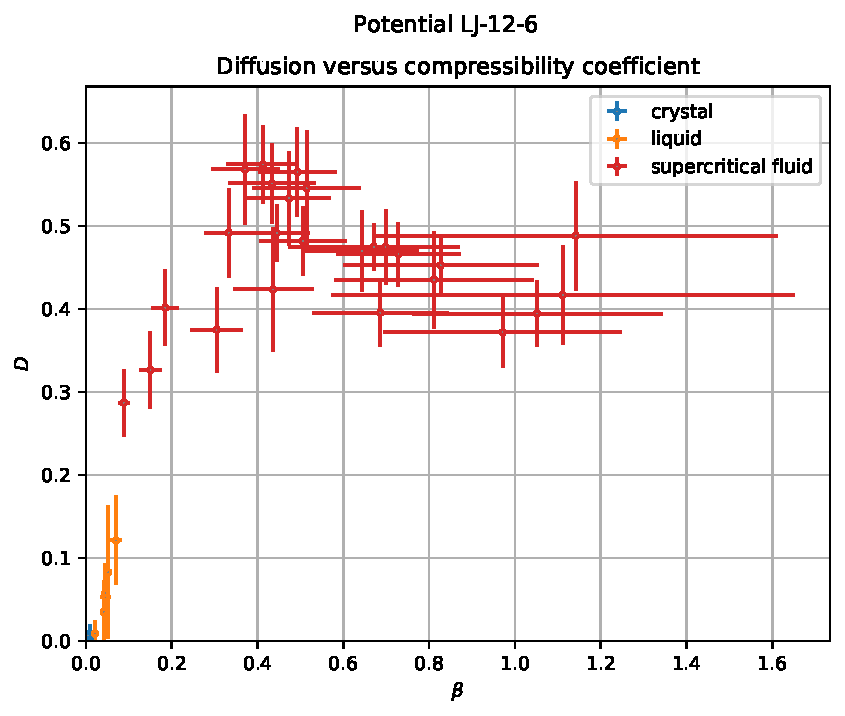
\includegraphics[width=\textwidth, keepaspectratio]{plot_diffusion_compress_Potential LJ-12-6_1}
\end{minipage}
\caption{Зависимость диффузии от сжимаемости. Не доделана!}
\label{risDBeta}
\end{center}
\end{figure}



\begin{figure}[h]
\begin{center}
\begin{minipage}[h]{0.45\linewidth}
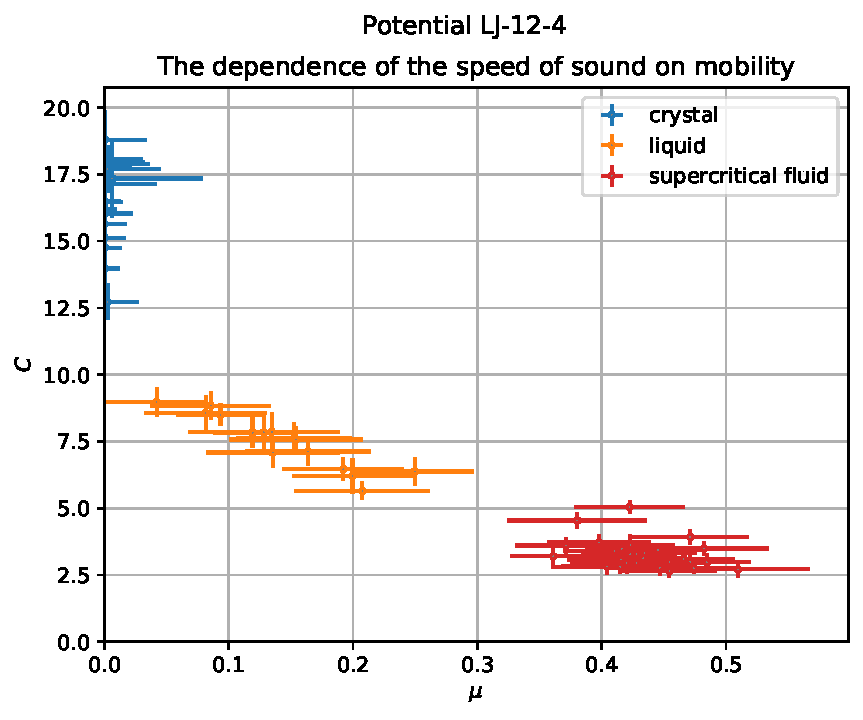
\includegraphics[width=\textwidth, keepaspectratio]{sound_speed_mobility_Potential LJ-12-4_1}
\end{minipage}
%\hfill
\begin{minipage}[h]{0.45\linewidth}
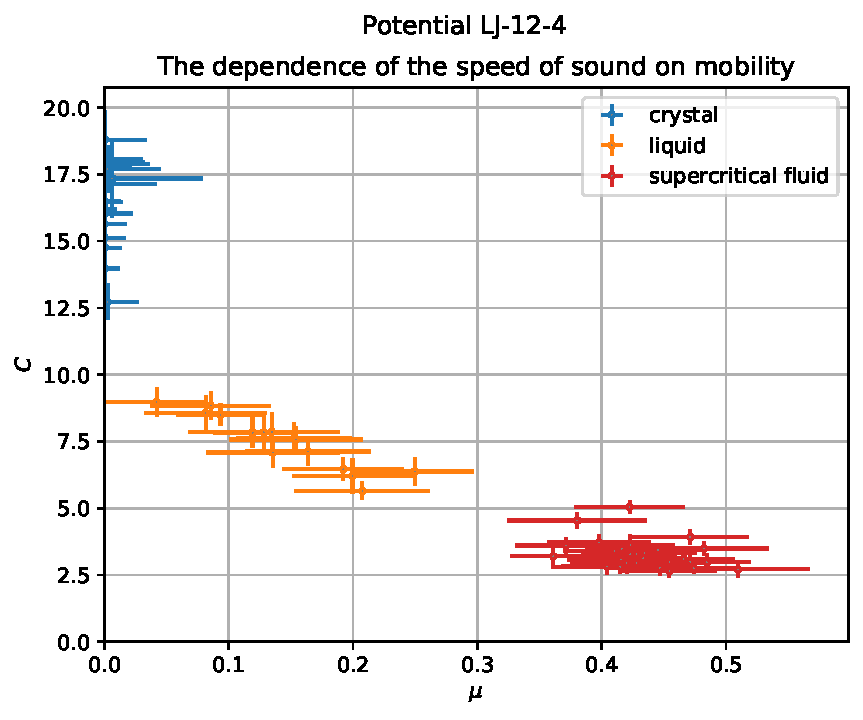
\includegraphics[width=\textwidth, keepaspectratio]{sound_speed_mobility_Potential LJ-12-4_1}
\end{minipage}

\begin{minipage}[h]{0.45\linewidth}
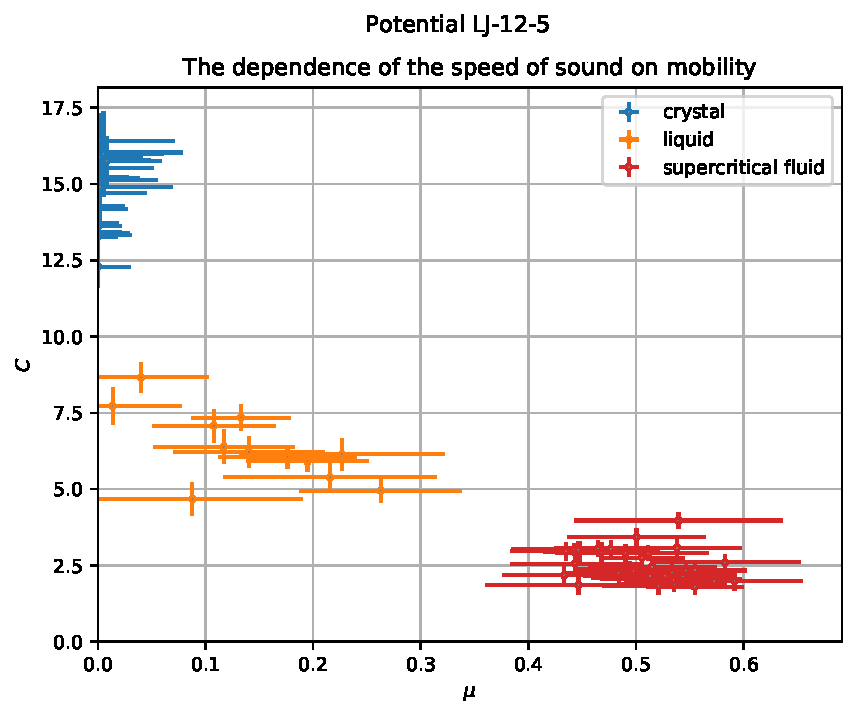
\includegraphics[width=\textwidth, keepaspectratio]{sound_speed_mobility_Potential LJ-12-5_1}
\end{minipage}
%\hfill
\begin{minipage}[h]{0.45\linewidth}
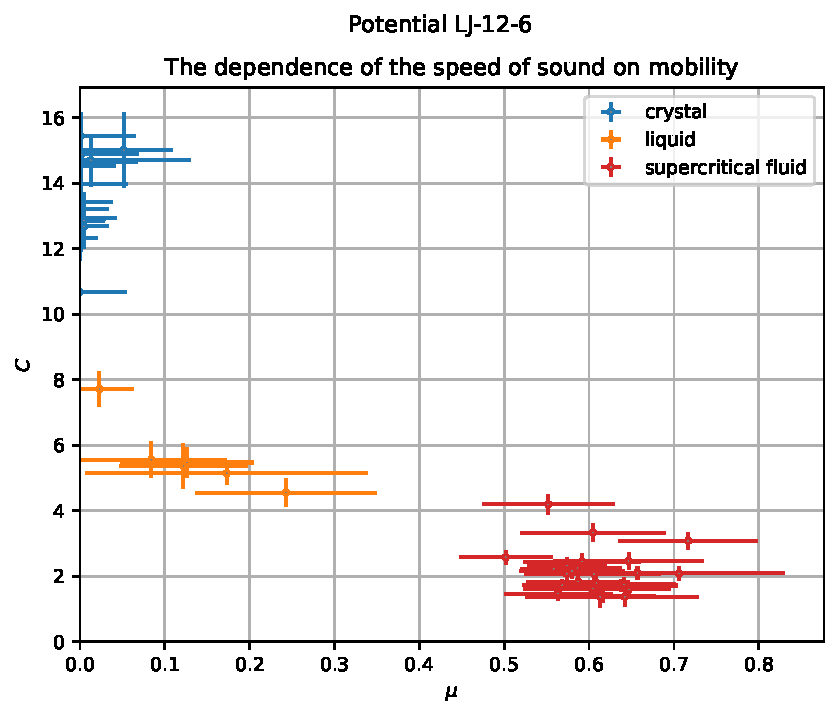
\includegraphics[width=\textwidth, keepaspectratio]{sound_speed_mobility_Potential LJ-12-6_1}
\end{minipage}
\caption{Зависимость скорости звука от мобильности. Не доделана!}
\label{risCMu}
\end{center}
\end{figure}

На примере рисунка \ref{risCMu} видно, что по совокупности параметров скорости звука и подвижности частиц система отчетливо делится на три класса, точки, которые принадлежат кристаллической фазе, жидкой, и за критической точкой. 

Такое четкое различие в расположениях точек дает возможность использовать различные классификаторы, например нейронные сети для определения принадлежности определенных точек к той или иной фазе. 


\section{Выводы главы}\label{C3_3}

В данной главе были рассмотрены расчеты диффузии методами молекулярной динамики, и его особенности. Данный метод, в совокупности с методом распознавания фаз, описанном в разделе \ref{C2_1}, позволяет достаточно точно определить подвижность частиц в конденсированной фазе, а так же ее температурную зависимость.

Выявлено влияние изменения температуры на подвижность частиц, в зависимости от дальнодействия притяжения.

Предложен метод классификации системы на конденсат, жидкость и сверхкритическую жидкость с использованием нейронных сетей.

\newpage
\newpage
\begin{center}
\textbf{\large ВЫВОДЫ РАБОТЫ}
\end{center}
\refstepcounter{chapter}


% \section*{}
\addcontentsline{toc}{chapter}{ВЫВОДЫ РАБОТЫ}

В данной работе рассмотрены методы изучения молекулярных систем, которые, используя только координаты частиц в разные моменты времени, позволяют узнать некоторые термодинамические параметры системы, а так же довольно точно определять критические точки в веществах. 

Было показано, каким образом можно эффективно классифицировать частицы на газ, конденсат и поверхность, с помощью разбиение системы на ячейки вороного. Была проведена модернизация алгоритма классификации, которая позволяет улучшить качество распознавания фаз, и убрать артефакты из статистики распределений по ячейкам различных величин.

Разработан и автоматизирован метод, позволяющий определять критические точки в веществе с удовлетворительной точностью.

Установлена роль притяжения в расположении тройных и критических точек, а также точек с наибольшими флуктуациями плотности в системе.

Предложен способ определения сжимаемости и скорости звука в веществе, используя только распределение плотностей ячеек вороного, а так же способ определения линии Видома для плотности, с помощью моментов величины плотности вещества.

Кроме того, в данной работе было выяснено влияние дальнодействия притяжения на подвижность частиц в веществе, и их температурные зависимости. Предложен способ классификации системы на кристалл, жидкость и сверхкритическую жидкость с помощью нейронных сетей, по параметрам скорости звука и мобильности в веществе.

\newpage
%\setcounter{chapter}{0}


\newpage
%\addcontentsline{toc}{chapter}{СПИСОК ИСПОЛЬЗОВАННЫХ ИСТОЧНИКОВ}
%\bibliographystyle{ugost2008}
\bibliography{Bak}

%\bibliographystyle{plain}
%\bibliography{Notesonreferences}

\end{document}